\documentclass[12pt]{book}
\usepackage{docmute}
\usepackage[backend=biber, style=numeric, natbib=true, maxcitenames=1, backend=biber, sorting=nyt, autolang=hyphen]{biblatex}
\usepackage[siunitx,europeanresistors,nooldvoltagedirection]{circuitikz}
\usetikzlibrary{calc,positioning,backgrounds}
\usepackage{import}
 \usepackage{listings}
\usepackage{subcaption}
\usepackage{url}

% Define local constants, that will be removed when imported into the main file
\addbibresource[location=local]{../bibliography.bib}

% Define constants here
\ctikzset{
  amplifiers/fill=cyan!25,
  sources/fill=green!70!black,
  csources/fill=green!70!black,
  diodes/fill=red,
  resistors/fill=blue!25,
}
\ctikzloadstyle{romano}

\providecommand{\device}[1]{\texttt{\small #1}}

\begin{document}
\section{Simulating Current Source Properties in LTSpice}
\label{sec:ltspice_current_source}
This section explains some more advanced concepts of LTSpice \cite{ltspice} to simulate device properties and circuit properties used when working with the current source presented in section \ref{sec:precision_current_source}. This section does not aim at explaining the basic functions of LTSpice, but rather some special functions. It is left to the interested reader to acquire those basic skills. The example presented here, allows to generate the MOSFET \textit{Typical Output Characteristics} plot found in datasheets, the transconductance of a MOSFET and the (dynamic) output impedance of a current source. The typical output characteristics can be used to compare the model with the datasheet or with measurements taken. Comparing these model parameters with the datasheet can establish confidence, that the simulation results can be transferred to a real circuit.

\subsection{MOSFET Typical Output Characteristics}
The output characterisic is a graph found in all MOSFET datasheets and is shown below in figure \ref{fig:ltspice_mosfet_drain_current_example}.

\begin{figure}[hb]
    \centering
    %% Creator: Matplotlib, PGF backend
%%
%% To include the figure in your LaTeX document, write
%%   \input{<filename>.pgf}
%%
%% Make sure the required packages are loaded in your preamble
%%   \usepackage{pgf}
%%
%% Also ensure that all the required font packages are loaded; for instance,
%% the lmodern package is sometimes necessary when using math font.
%%   \usepackage{lmodern}
%%
%% Figures using additional raster images can only be included by \input if
%% they are in the same directory as the main LaTeX file. For loading figures
%% from other directories you can use the `import` package
%%   \usepackage{import}
%%
%% and then include the figures with
%%   \import{<path to file>}{<filename>.pgf}
%%
%% Matplotlib used the following preamble
%%   \def\mathdefault#1{#1}
%%   \everymath=\expandafter{\the\everymath\displaystyle}
%%   \usepackage{siunitx}
%%   \sisetup{per-mode = symbol}%
%%   \ifdefined\pdftexversion\else  % non-pdftex case.
%%     \usepackage{fontspec}
%%   \fi
%%   \makeatletter\@ifpackageloaded{underscore}{}{\usepackage[strings]{underscore}}\makeatother
%%
\begingroup%
\makeatletter%
\begin{pgfpicture}%
\pgfpathrectangle{\pgfpointorigin}{\pgfqpoint{5.431103in}{3.356606in}}%
\pgfusepath{use as bounding box, clip}%
\begin{pgfscope}%
\pgfsetbuttcap%
\pgfsetmiterjoin%
\definecolor{currentfill}{rgb}{1.000000,1.000000,1.000000}%
\pgfsetfillcolor{currentfill}%
\pgfsetlinewidth{0.000000pt}%
\definecolor{currentstroke}{rgb}{1.000000,1.000000,1.000000}%
\pgfsetstrokecolor{currentstroke}%
\pgfsetdash{}{0pt}%
\pgfpathmoveto{\pgfqpoint{0.000000in}{0.000000in}}%
\pgfpathlineto{\pgfqpoint{5.431103in}{0.000000in}}%
\pgfpathlineto{\pgfqpoint{5.431103in}{3.356606in}}%
\pgfpathlineto{\pgfqpoint{0.000000in}{3.356606in}}%
\pgfpathlineto{\pgfqpoint{0.000000in}{0.000000in}}%
\pgfpathclose%
\pgfusepath{fill}%
\end{pgfscope}%
\begin{pgfscope}%
\pgfsetbuttcap%
\pgfsetmiterjoin%
\definecolor{currentfill}{rgb}{1.000000,1.000000,1.000000}%
\pgfsetfillcolor{currentfill}%
\pgfsetlinewidth{0.000000pt}%
\definecolor{currentstroke}{rgb}{0.000000,0.000000,0.000000}%
\pgfsetstrokecolor{currentstroke}%
\pgfsetstrokeopacity{0.000000}%
\pgfsetdash{}{0pt}%
\pgfpathmoveto{\pgfqpoint{0.693677in}{0.524170in}}%
\pgfpathlineto{\pgfqpoint{5.281103in}{0.524170in}}%
\pgfpathlineto{\pgfqpoint{5.281103in}{3.082363in}}%
\pgfpathlineto{\pgfqpoint{0.693677in}{3.082363in}}%
\pgfpathlineto{\pgfqpoint{0.693677in}{0.524170in}}%
\pgfpathclose%
\pgfusepath{fill}%
\end{pgfscope}%
\begin{pgfscope}%
\pgfpathrectangle{\pgfqpoint{0.693677in}{0.524170in}}{\pgfqpoint{4.587426in}{2.558193in}}%
\pgfusepath{clip}%
\pgfsetrectcap%
\pgfsetroundjoin%
\pgfsetlinewidth{0.803000pt}%
\definecolor{currentstroke}{rgb}{0.450000,0.450000,0.450000}%
\pgfsetstrokecolor{currentstroke}%
\pgfsetdash{}{0pt}%
\pgfpathmoveto{\pgfqpoint{5.072583in}{0.524170in}}%
\pgfpathlineto{\pgfqpoint{5.072583in}{3.082363in}}%
\pgfusepath{stroke}%
\end{pgfscope}%
\begin{pgfscope}%
\pgfsetbuttcap%
\pgfsetroundjoin%
\definecolor{currentfill}{rgb}{0.000000,0.000000,0.000000}%
\pgfsetfillcolor{currentfill}%
\pgfsetlinewidth{0.803000pt}%
\definecolor{currentstroke}{rgb}{0.000000,0.000000,0.000000}%
\pgfsetstrokecolor{currentstroke}%
\pgfsetdash{}{0pt}%
\pgfsys@defobject{currentmarker}{\pgfqpoint{0.000000in}{-0.048611in}}{\pgfqpoint{0.000000in}{0.000000in}}{%
\pgfpathmoveto{\pgfqpoint{0.000000in}{0.000000in}}%
\pgfpathlineto{\pgfqpoint{0.000000in}{-0.048611in}}%
\pgfusepath{stroke,fill}%
}%
\begin{pgfscope}%
\pgfsys@transformshift{5.072583in}{0.524170in}%
\pgfsys@useobject{currentmarker}{}%
\end{pgfscope}%
\end{pgfscope}%
\begin{pgfscope}%
\definecolor{textcolor}{rgb}{0.000000,0.000000,0.000000}%
\pgfsetstrokecolor{textcolor}%
\pgfsetfillcolor{textcolor}%
\pgftext[x=5.072583in,y=0.426948in,,top]{\color{textcolor}{\rmfamily\fontsize{8.000000}{9.600000}\selectfont\catcode`\^=\active\def^{\ifmmode\sp\else\^{}\fi}\catcode`\%=\active\def%{\%}$\mathdefault{\ensuremath{-}1.0}$}}%
\end{pgfscope}%
\begin{pgfscope}%
\pgfpathrectangle{\pgfqpoint{0.693677in}{0.524170in}}{\pgfqpoint{4.587426in}{2.558193in}}%
\pgfusepath{clip}%
\pgfsetrectcap%
\pgfsetroundjoin%
\pgfsetlinewidth{0.803000pt}%
\definecolor{currentstroke}{rgb}{0.450000,0.450000,0.450000}%
\pgfsetstrokecolor{currentstroke}%
\pgfsetdash{}{0pt}%
\pgfpathmoveto{\pgfqpoint{4.238506in}{0.524170in}}%
\pgfpathlineto{\pgfqpoint{4.238506in}{3.082363in}}%
\pgfusepath{stroke}%
\end{pgfscope}%
\begin{pgfscope}%
\pgfsetbuttcap%
\pgfsetroundjoin%
\definecolor{currentfill}{rgb}{0.000000,0.000000,0.000000}%
\pgfsetfillcolor{currentfill}%
\pgfsetlinewidth{0.803000pt}%
\definecolor{currentstroke}{rgb}{0.000000,0.000000,0.000000}%
\pgfsetstrokecolor{currentstroke}%
\pgfsetdash{}{0pt}%
\pgfsys@defobject{currentmarker}{\pgfqpoint{0.000000in}{-0.048611in}}{\pgfqpoint{0.000000in}{0.000000in}}{%
\pgfpathmoveto{\pgfqpoint{0.000000in}{0.000000in}}%
\pgfpathlineto{\pgfqpoint{0.000000in}{-0.048611in}}%
\pgfusepath{stroke,fill}%
}%
\begin{pgfscope}%
\pgfsys@transformshift{4.238506in}{0.524170in}%
\pgfsys@useobject{currentmarker}{}%
\end{pgfscope}%
\end{pgfscope}%
\begin{pgfscope}%
\definecolor{textcolor}{rgb}{0.000000,0.000000,0.000000}%
\pgfsetstrokecolor{textcolor}%
\pgfsetfillcolor{textcolor}%
\pgftext[x=4.238506in,y=0.426948in,,top]{\color{textcolor}{\rmfamily\fontsize{8.000000}{9.600000}\selectfont\catcode`\^=\active\def^{\ifmmode\sp\else\^{}\fi}\catcode`\%=\active\def%{\%}$\mathdefault{\ensuremath{-}0.8}$}}%
\end{pgfscope}%
\begin{pgfscope}%
\pgfpathrectangle{\pgfqpoint{0.693677in}{0.524170in}}{\pgfqpoint{4.587426in}{2.558193in}}%
\pgfusepath{clip}%
\pgfsetrectcap%
\pgfsetroundjoin%
\pgfsetlinewidth{0.803000pt}%
\definecolor{currentstroke}{rgb}{0.450000,0.450000,0.450000}%
\pgfsetstrokecolor{currentstroke}%
\pgfsetdash{}{0pt}%
\pgfpathmoveto{\pgfqpoint{3.404428in}{0.524170in}}%
\pgfpathlineto{\pgfqpoint{3.404428in}{3.082363in}}%
\pgfusepath{stroke}%
\end{pgfscope}%
\begin{pgfscope}%
\pgfsetbuttcap%
\pgfsetroundjoin%
\definecolor{currentfill}{rgb}{0.000000,0.000000,0.000000}%
\pgfsetfillcolor{currentfill}%
\pgfsetlinewidth{0.803000pt}%
\definecolor{currentstroke}{rgb}{0.000000,0.000000,0.000000}%
\pgfsetstrokecolor{currentstroke}%
\pgfsetdash{}{0pt}%
\pgfsys@defobject{currentmarker}{\pgfqpoint{0.000000in}{-0.048611in}}{\pgfqpoint{0.000000in}{0.000000in}}{%
\pgfpathmoveto{\pgfqpoint{0.000000in}{0.000000in}}%
\pgfpathlineto{\pgfqpoint{0.000000in}{-0.048611in}}%
\pgfusepath{stroke,fill}%
}%
\begin{pgfscope}%
\pgfsys@transformshift{3.404428in}{0.524170in}%
\pgfsys@useobject{currentmarker}{}%
\end{pgfscope}%
\end{pgfscope}%
\begin{pgfscope}%
\definecolor{textcolor}{rgb}{0.000000,0.000000,0.000000}%
\pgfsetstrokecolor{textcolor}%
\pgfsetfillcolor{textcolor}%
\pgftext[x=3.404428in,y=0.426948in,,top]{\color{textcolor}{\rmfamily\fontsize{8.000000}{9.600000}\selectfont\catcode`\^=\active\def^{\ifmmode\sp\else\^{}\fi}\catcode`\%=\active\def%{\%}$\mathdefault{\ensuremath{-}0.6}$}}%
\end{pgfscope}%
\begin{pgfscope}%
\pgfpathrectangle{\pgfqpoint{0.693677in}{0.524170in}}{\pgfqpoint{4.587426in}{2.558193in}}%
\pgfusepath{clip}%
\pgfsetrectcap%
\pgfsetroundjoin%
\pgfsetlinewidth{0.803000pt}%
\definecolor{currentstroke}{rgb}{0.450000,0.450000,0.450000}%
\pgfsetstrokecolor{currentstroke}%
\pgfsetdash{}{0pt}%
\pgfpathmoveto{\pgfqpoint{2.570351in}{0.524170in}}%
\pgfpathlineto{\pgfqpoint{2.570351in}{3.082363in}}%
\pgfusepath{stroke}%
\end{pgfscope}%
\begin{pgfscope}%
\pgfsetbuttcap%
\pgfsetroundjoin%
\definecolor{currentfill}{rgb}{0.000000,0.000000,0.000000}%
\pgfsetfillcolor{currentfill}%
\pgfsetlinewidth{0.803000pt}%
\definecolor{currentstroke}{rgb}{0.000000,0.000000,0.000000}%
\pgfsetstrokecolor{currentstroke}%
\pgfsetdash{}{0pt}%
\pgfsys@defobject{currentmarker}{\pgfqpoint{0.000000in}{-0.048611in}}{\pgfqpoint{0.000000in}{0.000000in}}{%
\pgfpathmoveto{\pgfqpoint{0.000000in}{0.000000in}}%
\pgfpathlineto{\pgfqpoint{0.000000in}{-0.048611in}}%
\pgfusepath{stroke,fill}%
}%
\begin{pgfscope}%
\pgfsys@transformshift{2.570351in}{0.524170in}%
\pgfsys@useobject{currentmarker}{}%
\end{pgfscope}%
\end{pgfscope}%
\begin{pgfscope}%
\definecolor{textcolor}{rgb}{0.000000,0.000000,0.000000}%
\pgfsetstrokecolor{textcolor}%
\pgfsetfillcolor{textcolor}%
\pgftext[x=2.570351in,y=0.426948in,,top]{\color{textcolor}{\rmfamily\fontsize{8.000000}{9.600000}\selectfont\catcode`\^=\active\def^{\ifmmode\sp\else\^{}\fi}\catcode`\%=\active\def%{\%}$\mathdefault{\ensuremath{-}0.4}$}}%
\end{pgfscope}%
\begin{pgfscope}%
\pgfpathrectangle{\pgfqpoint{0.693677in}{0.524170in}}{\pgfqpoint{4.587426in}{2.558193in}}%
\pgfusepath{clip}%
\pgfsetrectcap%
\pgfsetroundjoin%
\pgfsetlinewidth{0.803000pt}%
\definecolor{currentstroke}{rgb}{0.450000,0.450000,0.450000}%
\pgfsetstrokecolor{currentstroke}%
\pgfsetdash{}{0pt}%
\pgfpathmoveto{\pgfqpoint{1.736274in}{0.524170in}}%
\pgfpathlineto{\pgfqpoint{1.736274in}{3.082363in}}%
\pgfusepath{stroke}%
\end{pgfscope}%
\begin{pgfscope}%
\pgfsetbuttcap%
\pgfsetroundjoin%
\definecolor{currentfill}{rgb}{0.000000,0.000000,0.000000}%
\pgfsetfillcolor{currentfill}%
\pgfsetlinewidth{0.803000pt}%
\definecolor{currentstroke}{rgb}{0.000000,0.000000,0.000000}%
\pgfsetstrokecolor{currentstroke}%
\pgfsetdash{}{0pt}%
\pgfsys@defobject{currentmarker}{\pgfqpoint{0.000000in}{-0.048611in}}{\pgfqpoint{0.000000in}{0.000000in}}{%
\pgfpathmoveto{\pgfqpoint{0.000000in}{0.000000in}}%
\pgfpathlineto{\pgfqpoint{0.000000in}{-0.048611in}}%
\pgfusepath{stroke,fill}%
}%
\begin{pgfscope}%
\pgfsys@transformshift{1.736274in}{0.524170in}%
\pgfsys@useobject{currentmarker}{}%
\end{pgfscope}%
\end{pgfscope}%
\begin{pgfscope}%
\definecolor{textcolor}{rgb}{0.000000,0.000000,0.000000}%
\pgfsetstrokecolor{textcolor}%
\pgfsetfillcolor{textcolor}%
\pgftext[x=1.736274in,y=0.426948in,,top]{\color{textcolor}{\rmfamily\fontsize{8.000000}{9.600000}\selectfont\catcode`\^=\active\def^{\ifmmode\sp\else\^{}\fi}\catcode`\%=\active\def%{\%}$\mathdefault{\ensuremath{-}0.2}$}}%
\end{pgfscope}%
\begin{pgfscope}%
\pgfpathrectangle{\pgfqpoint{0.693677in}{0.524170in}}{\pgfqpoint{4.587426in}{2.558193in}}%
\pgfusepath{clip}%
\pgfsetrectcap%
\pgfsetroundjoin%
\pgfsetlinewidth{0.803000pt}%
\definecolor{currentstroke}{rgb}{0.450000,0.450000,0.450000}%
\pgfsetstrokecolor{currentstroke}%
\pgfsetdash{}{0pt}%
\pgfpathmoveto{\pgfqpoint{0.902196in}{0.524170in}}%
\pgfpathlineto{\pgfqpoint{0.902196in}{3.082363in}}%
\pgfusepath{stroke}%
\end{pgfscope}%
\begin{pgfscope}%
\pgfsetbuttcap%
\pgfsetroundjoin%
\definecolor{currentfill}{rgb}{0.000000,0.000000,0.000000}%
\pgfsetfillcolor{currentfill}%
\pgfsetlinewidth{0.803000pt}%
\definecolor{currentstroke}{rgb}{0.000000,0.000000,0.000000}%
\pgfsetstrokecolor{currentstroke}%
\pgfsetdash{}{0pt}%
\pgfsys@defobject{currentmarker}{\pgfqpoint{0.000000in}{-0.048611in}}{\pgfqpoint{0.000000in}{0.000000in}}{%
\pgfpathmoveto{\pgfqpoint{0.000000in}{0.000000in}}%
\pgfpathlineto{\pgfqpoint{0.000000in}{-0.048611in}}%
\pgfusepath{stroke,fill}%
}%
\begin{pgfscope}%
\pgfsys@transformshift{0.902196in}{0.524170in}%
\pgfsys@useobject{currentmarker}{}%
\end{pgfscope}%
\end{pgfscope}%
\begin{pgfscope}%
\definecolor{textcolor}{rgb}{0.000000,0.000000,0.000000}%
\pgfsetstrokecolor{textcolor}%
\pgfsetfillcolor{textcolor}%
\pgftext[x=0.902196in,y=0.426948in,,top]{\color{textcolor}{\rmfamily\fontsize{8.000000}{9.600000}\selectfont\catcode`\^=\active\def^{\ifmmode\sp\else\^{}\fi}\catcode`\%=\active\def%{\%}$\mathdefault{0.0}$}}%
\end{pgfscope}%
\begin{pgfscope}%
\definecolor{textcolor}{rgb}{0.000000,0.000000,0.000000}%
\pgfsetstrokecolor{textcolor}%
\pgfsetfillcolor{textcolor}%
\pgftext[x=2.987390in,y=0.272725in,,top]{\color{textcolor}{\rmfamily\fontsize{10.000000}{12.000000}\selectfont\catcode`\^=\active\def^{\ifmmode\sp\else\^{}\fi}\catcode`\%=\active\def%{\%}Drain-source voltage $V_{DS}$ in \unit{\V}}}%
\end{pgfscope}%
\begin{pgfscope}%
\pgfpathrectangle{\pgfqpoint{0.693677in}{0.524170in}}{\pgfqpoint{4.587426in}{2.558193in}}%
\pgfusepath{clip}%
\pgfsetrectcap%
\pgfsetroundjoin%
\pgfsetlinewidth{0.803000pt}%
\definecolor{currentstroke}{rgb}{0.450000,0.450000,0.450000}%
\pgfsetstrokecolor{currentstroke}%
\pgfsetdash{}{0pt}%
\pgfpathmoveto{\pgfqpoint{0.693677in}{2.866355in}}%
\pgfpathlineto{\pgfqpoint{5.281103in}{2.866355in}}%
\pgfusepath{stroke}%
\end{pgfscope}%
\begin{pgfscope}%
\pgfsetbuttcap%
\pgfsetroundjoin%
\definecolor{currentfill}{rgb}{0.000000,0.000000,0.000000}%
\pgfsetfillcolor{currentfill}%
\pgfsetlinewidth{0.803000pt}%
\definecolor{currentstroke}{rgb}{0.000000,0.000000,0.000000}%
\pgfsetstrokecolor{currentstroke}%
\pgfsetdash{}{0pt}%
\pgfsys@defobject{currentmarker}{\pgfqpoint{-0.048611in}{0.000000in}}{\pgfqpoint{-0.000000in}{0.000000in}}{%
\pgfpathmoveto{\pgfqpoint{-0.000000in}{0.000000in}}%
\pgfpathlineto{\pgfqpoint{-0.048611in}{0.000000in}}%
\pgfusepath{stroke,fill}%
}%
\begin{pgfscope}%
\pgfsys@transformshift{0.693677in}{2.866355in}%
\pgfsys@useobject{currentmarker}{}%
\end{pgfscope}%
\end{pgfscope}%
\begin{pgfscope}%
\definecolor{textcolor}{rgb}{0.000000,0.000000,0.000000}%
\pgfsetstrokecolor{textcolor}%
\pgfsetfillcolor{textcolor}%
\pgftext[x=0.327546in, y=2.827800in, left, base]{\color{textcolor}{\rmfamily\fontsize{8.000000}{9.600000}\selectfont\catcode`\^=\active\def^{\ifmmode\sp\else\^{}\fi}\catcode`\%=\active\def%{\%}$\mathdefault{\ensuremath{-}250}$}}%
\end{pgfscope}%
\begin{pgfscope}%
\pgfpathrectangle{\pgfqpoint{0.693677in}{0.524170in}}{\pgfqpoint{4.587426in}{2.558193in}}%
\pgfusepath{clip}%
\pgfsetrectcap%
\pgfsetroundjoin%
\pgfsetlinewidth{0.803000pt}%
\definecolor{currentstroke}{rgb}{0.450000,0.450000,0.450000}%
\pgfsetstrokecolor{currentstroke}%
\pgfsetdash{}{0pt}%
\pgfpathmoveto{\pgfqpoint{0.693677in}{2.421174in}}%
\pgfpathlineto{\pgfqpoint{5.281103in}{2.421174in}}%
\pgfusepath{stroke}%
\end{pgfscope}%
\begin{pgfscope}%
\pgfsetbuttcap%
\pgfsetroundjoin%
\definecolor{currentfill}{rgb}{0.000000,0.000000,0.000000}%
\pgfsetfillcolor{currentfill}%
\pgfsetlinewidth{0.803000pt}%
\definecolor{currentstroke}{rgb}{0.000000,0.000000,0.000000}%
\pgfsetstrokecolor{currentstroke}%
\pgfsetdash{}{0pt}%
\pgfsys@defobject{currentmarker}{\pgfqpoint{-0.048611in}{0.000000in}}{\pgfqpoint{-0.000000in}{0.000000in}}{%
\pgfpathmoveto{\pgfqpoint{-0.000000in}{0.000000in}}%
\pgfpathlineto{\pgfqpoint{-0.048611in}{0.000000in}}%
\pgfusepath{stroke,fill}%
}%
\begin{pgfscope}%
\pgfsys@transformshift{0.693677in}{2.421174in}%
\pgfsys@useobject{currentmarker}{}%
\end{pgfscope}%
\end{pgfscope}%
\begin{pgfscope}%
\definecolor{textcolor}{rgb}{0.000000,0.000000,0.000000}%
\pgfsetstrokecolor{textcolor}%
\pgfsetfillcolor{textcolor}%
\pgftext[x=0.327546in, y=2.382619in, left, base]{\color{textcolor}{\rmfamily\fontsize{8.000000}{9.600000}\selectfont\catcode`\^=\active\def^{\ifmmode\sp\else\^{}\fi}\catcode`\%=\active\def%{\%}$\mathdefault{\ensuremath{-}200}$}}%
\end{pgfscope}%
\begin{pgfscope}%
\pgfpathrectangle{\pgfqpoint{0.693677in}{0.524170in}}{\pgfqpoint{4.587426in}{2.558193in}}%
\pgfusepath{clip}%
\pgfsetrectcap%
\pgfsetroundjoin%
\pgfsetlinewidth{0.803000pt}%
\definecolor{currentstroke}{rgb}{0.450000,0.450000,0.450000}%
\pgfsetstrokecolor{currentstroke}%
\pgfsetdash{}{0pt}%
\pgfpathmoveto{\pgfqpoint{0.693677in}{1.975994in}}%
\pgfpathlineto{\pgfqpoint{5.281103in}{1.975994in}}%
\pgfusepath{stroke}%
\end{pgfscope}%
\begin{pgfscope}%
\pgfsetbuttcap%
\pgfsetroundjoin%
\definecolor{currentfill}{rgb}{0.000000,0.000000,0.000000}%
\pgfsetfillcolor{currentfill}%
\pgfsetlinewidth{0.803000pt}%
\definecolor{currentstroke}{rgb}{0.000000,0.000000,0.000000}%
\pgfsetstrokecolor{currentstroke}%
\pgfsetdash{}{0pt}%
\pgfsys@defobject{currentmarker}{\pgfqpoint{-0.048611in}{0.000000in}}{\pgfqpoint{-0.000000in}{0.000000in}}{%
\pgfpathmoveto{\pgfqpoint{-0.000000in}{0.000000in}}%
\pgfpathlineto{\pgfqpoint{-0.048611in}{0.000000in}}%
\pgfusepath{stroke,fill}%
}%
\begin{pgfscope}%
\pgfsys@transformshift{0.693677in}{1.975994in}%
\pgfsys@useobject{currentmarker}{}%
\end{pgfscope}%
\end{pgfscope}%
\begin{pgfscope}%
\definecolor{textcolor}{rgb}{0.000000,0.000000,0.000000}%
\pgfsetstrokecolor{textcolor}%
\pgfsetfillcolor{textcolor}%
\pgftext[x=0.327546in, y=1.937438in, left, base]{\color{textcolor}{\rmfamily\fontsize{8.000000}{9.600000}\selectfont\catcode`\^=\active\def^{\ifmmode\sp\else\^{}\fi}\catcode`\%=\active\def%{\%}$\mathdefault{\ensuremath{-}150}$}}%
\end{pgfscope}%
\begin{pgfscope}%
\pgfpathrectangle{\pgfqpoint{0.693677in}{0.524170in}}{\pgfqpoint{4.587426in}{2.558193in}}%
\pgfusepath{clip}%
\pgfsetrectcap%
\pgfsetroundjoin%
\pgfsetlinewidth{0.803000pt}%
\definecolor{currentstroke}{rgb}{0.450000,0.450000,0.450000}%
\pgfsetstrokecolor{currentstroke}%
\pgfsetdash{}{0pt}%
\pgfpathmoveto{\pgfqpoint{0.693677in}{1.530813in}}%
\pgfpathlineto{\pgfqpoint{5.281103in}{1.530813in}}%
\pgfusepath{stroke}%
\end{pgfscope}%
\begin{pgfscope}%
\pgfsetbuttcap%
\pgfsetroundjoin%
\definecolor{currentfill}{rgb}{0.000000,0.000000,0.000000}%
\pgfsetfillcolor{currentfill}%
\pgfsetlinewidth{0.803000pt}%
\definecolor{currentstroke}{rgb}{0.000000,0.000000,0.000000}%
\pgfsetstrokecolor{currentstroke}%
\pgfsetdash{}{0pt}%
\pgfsys@defobject{currentmarker}{\pgfqpoint{-0.048611in}{0.000000in}}{\pgfqpoint{-0.000000in}{0.000000in}}{%
\pgfpathmoveto{\pgfqpoint{-0.000000in}{0.000000in}}%
\pgfpathlineto{\pgfqpoint{-0.048611in}{0.000000in}}%
\pgfusepath{stroke,fill}%
}%
\begin{pgfscope}%
\pgfsys@transformshift{0.693677in}{1.530813in}%
\pgfsys@useobject{currentmarker}{}%
\end{pgfscope}%
\end{pgfscope}%
\begin{pgfscope}%
\definecolor{textcolor}{rgb}{0.000000,0.000000,0.000000}%
\pgfsetstrokecolor{textcolor}%
\pgfsetfillcolor{textcolor}%
\pgftext[x=0.327546in, y=1.492257in, left, base]{\color{textcolor}{\rmfamily\fontsize{8.000000}{9.600000}\selectfont\catcode`\^=\active\def^{\ifmmode\sp\else\^{}\fi}\catcode`\%=\active\def%{\%}$\mathdefault{\ensuremath{-}100}$}}%
\end{pgfscope}%
\begin{pgfscope}%
\pgfpathrectangle{\pgfqpoint{0.693677in}{0.524170in}}{\pgfqpoint{4.587426in}{2.558193in}}%
\pgfusepath{clip}%
\pgfsetrectcap%
\pgfsetroundjoin%
\pgfsetlinewidth{0.803000pt}%
\definecolor{currentstroke}{rgb}{0.450000,0.450000,0.450000}%
\pgfsetstrokecolor{currentstroke}%
\pgfsetdash{}{0pt}%
\pgfpathmoveto{\pgfqpoint{0.693677in}{1.085632in}}%
\pgfpathlineto{\pgfqpoint{5.281103in}{1.085632in}}%
\pgfusepath{stroke}%
\end{pgfscope}%
\begin{pgfscope}%
\pgfsetbuttcap%
\pgfsetroundjoin%
\definecolor{currentfill}{rgb}{0.000000,0.000000,0.000000}%
\pgfsetfillcolor{currentfill}%
\pgfsetlinewidth{0.803000pt}%
\definecolor{currentstroke}{rgb}{0.000000,0.000000,0.000000}%
\pgfsetstrokecolor{currentstroke}%
\pgfsetdash{}{0pt}%
\pgfsys@defobject{currentmarker}{\pgfqpoint{-0.048611in}{0.000000in}}{\pgfqpoint{-0.000000in}{0.000000in}}{%
\pgfpathmoveto{\pgfqpoint{-0.000000in}{0.000000in}}%
\pgfpathlineto{\pgfqpoint{-0.048611in}{0.000000in}}%
\pgfusepath{stroke,fill}%
}%
\begin{pgfscope}%
\pgfsys@transformshift{0.693677in}{1.085632in}%
\pgfsys@useobject{currentmarker}{}%
\end{pgfscope}%
\end{pgfscope}%
\begin{pgfscope}%
\definecolor{textcolor}{rgb}{0.000000,0.000000,0.000000}%
\pgfsetstrokecolor{textcolor}%
\pgfsetfillcolor{textcolor}%
\pgftext[x=0.386575in, y=1.047076in, left, base]{\color{textcolor}{\rmfamily\fontsize{8.000000}{9.600000}\selectfont\catcode`\^=\active\def^{\ifmmode\sp\else\^{}\fi}\catcode`\%=\active\def%{\%}$\mathdefault{\ensuremath{-}50}$}}%
\end{pgfscope}%
\begin{pgfscope}%
\pgfpathrectangle{\pgfqpoint{0.693677in}{0.524170in}}{\pgfqpoint{4.587426in}{2.558193in}}%
\pgfusepath{clip}%
\pgfsetrectcap%
\pgfsetroundjoin%
\pgfsetlinewidth{0.803000pt}%
\definecolor{currentstroke}{rgb}{0.450000,0.450000,0.450000}%
\pgfsetstrokecolor{currentstroke}%
\pgfsetdash{}{0pt}%
\pgfpathmoveto{\pgfqpoint{0.693677in}{0.640451in}}%
\pgfpathlineto{\pgfqpoint{5.281103in}{0.640451in}}%
\pgfusepath{stroke}%
\end{pgfscope}%
\begin{pgfscope}%
\pgfsetbuttcap%
\pgfsetroundjoin%
\definecolor{currentfill}{rgb}{0.000000,0.000000,0.000000}%
\pgfsetfillcolor{currentfill}%
\pgfsetlinewidth{0.803000pt}%
\definecolor{currentstroke}{rgb}{0.000000,0.000000,0.000000}%
\pgfsetstrokecolor{currentstroke}%
\pgfsetdash{}{0pt}%
\pgfsys@defobject{currentmarker}{\pgfqpoint{-0.048611in}{0.000000in}}{\pgfqpoint{-0.000000in}{0.000000in}}{%
\pgfpathmoveto{\pgfqpoint{-0.000000in}{0.000000in}}%
\pgfpathlineto{\pgfqpoint{-0.048611in}{0.000000in}}%
\pgfusepath{stroke,fill}%
}%
\begin{pgfscope}%
\pgfsys@transformshift{0.693677in}{0.640451in}%
\pgfsys@useobject{currentmarker}{}%
\end{pgfscope}%
\end{pgfscope}%
\begin{pgfscope}%
\definecolor{textcolor}{rgb}{0.000000,0.000000,0.000000}%
\pgfsetstrokecolor{textcolor}%
\pgfsetfillcolor{textcolor}%
\pgftext[x=0.537426in, y=0.601896in, left, base]{\color{textcolor}{\rmfamily\fontsize{8.000000}{9.600000}\selectfont\catcode`\^=\active\def^{\ifmmode\sp\else\^{}\fi}\catcode`\%=\active\def%{\%}$\mathdefault{0}$}}%
\end{pgfscope}%
\begin{pgfscope}%
\definecolor{textcolor}{rgb}{0.000000,0.000000,0.000000}%
\pgfsetstrokecolor{textcolor}%
\pgfsetfillcolor{textcolor}%
\pgftext[x=0.271991in,y=1.803266in,,bottom,rotate=90.000000]{\color{textcolor}{\rmfamily\fontsize{10.000000}{12.000000}\selectfont\catcode`\^=\active\def^{\ifmmode\sp\else\^{}\fi}\catcode`\%=\active\def%{\%}Drain Current $I_{D}$ in \unit{\A}}}%
\end{pgfscope}%
\begin{pgfscope}%
\definecolor{textcolor}{rgb}{0.000000,0.000000,0.000000}%
\pgfsetstrokecolor{textcolor}%
\pgfsetfillcolor{textcolor}%
\pgftext[x=0.693677in,y=3.124029in,left,base]{\color{textcolor}{\rmfamily\fontsize{8.000000}{9.600000}\selectfont\catcode`\^=\active\def^{\ifmmode\sp\else\^{}\fi}\catcode`\%=\active\def%{\%}$\times\mathdefault{10^{\ensuremath{-}3}}\mathdefault{}$}}%
\end{pgfscope}%
\begin{pgfscope}%
\pgfpathrectangle{\pgfqpoint{0.693677in}{0.524170in}}{\pgfqpoint{4.587426in}{2.558193in}}%
\pgfusepath{clip}%
\pgfsetrectcap%
\pgfsetroundjoin%
\pgfsetlinewidth{1.505625pt}%
\definecolor{currentstroke}{rgb}{0.003922,0.450980,0.698039}%
\pgfsetstrokecolor{currentstroke}%
\pgfsetstrokeopacity{0.700000}%
\pgfsetdash{}{0pt}%
\pgfpathmoveto{\pgfqpoint{0.902196in}{0.640451in}}%
\pgfpathlineto{\pgfqpoint{0.943900in}{0.654567in}}%
\pgfpathlineto{\pgfqpoint{0.985604in}{0.667960in}}%
\pgfpathlineto{\pgfqpoint{1.027308in}{0.680631in}}%
\pgfpathlineto{\pgfqpoint{1.069012in}{0.692578in}}%
\pgfpathlineto{\pgfqpoint{1.110716in}{0.703802in}}%
\pgfpathlineto{\pgfqpoint{1.152419in}{0.714303in}}%
\pgfpathlineto{\pgfqpoint{1.194123in}{0.724081in}}%
\pgfpathlineto{\pgfqpoint{1.235827in}{0.733136in}}%
\pgfpathlineto{\pgfqpoint{1.277531in}{0.741467in}}%
\pgfpathlineto{\pgfqpoint{1.319235in}{0.749074in}}%
\pgfpathlineto{\pgfqpoint{1.360939in}{0.755958in}}%
\pgfpathlineto{\pgfqpoint{1.402643in}{0.762119in}}%
\pgfpathlineto{\pgfqpoint{1.444346in}{0.767555in}}%
\pgfpathlineto{\pgfqpoint{1.486050in}{0.772268in}}%
\pgfpathlineto{\pgfqpoint{1.527754in}{0.776257in}}%
\pgfpathlineto{\pgfqpoint{1.569458in}{0.779522in}}%
\pgfpathlineto{\pgfqpoint{1.611162in}{0.782063in}}%
\pgfpathlineto{\pgfqpoint{1.652866in}{0.783880in}}%
\pgfpathlineto{\pgfqpoint{1.694570in}{0.784972in}}%
\pgfpathlineto{\pgfqpoint{1.736274in}{0.785340in}}%
\pgfpathlineto{\pgfqpoint{1.777977in}{0.785346in}}%
\pgfpathlineto{\pgfqpoint{1.819681in}{0.785351in}}%
\pgfpathlineto{\pgfqpoint{1.861385in}{0.785357in}}%
\pgfpathlineto{\pgfqpoint{1.903089in}{0.785363in}}%
\pgfpathlineto{\pgfqpoint{1.944793in}{0.785369in}}%
\pgfpathlineto{\pgfqpoint{1.986497in}{0.785375in}}%
\pgfpathlineto{\pgfqpoint{2.028201in}{0.785380in}}%
\pgfpathlineto{\pgfqpoint{2.069905in}{0.785386in}}%
\pgfpathlineto{\pgfqpoint{2.111608in}{0.785392in}}%
\pgfpathlineto{\pgfqpoint{2.153312in}{0.785398in}}%
\pgfpathlineto{\pgfqpoint{2.195016in}{0.785404in}}%
\pgfpathlineto{\pgfqpoint{2.236720in}{0.785409in}}%
\pgfpathlineto{\pgfqpoint{2.278424in}{0.785415in}}%
\pgfpathlineto{\pgfqpoint{2.320128in}{0.785421in}}%
\pgfpathlineto{\pgfqpoint{2.361832in}{0.785427in}}%
\pgfpathlineto{\pgfqpoint{2.403536in}{0.785433in}}%
\pgfpathlineto{\pgfqpoint{2.445239in}{0.785438in}}%
\pgfpathlineto{\pgfqpoint{2.486943in}{0.785444in}}%
\pgfpathlineto{\pgfqpoint{2.528647in}{0.785450in}}%
\pgfpathlineto{\pgfqpoint{2.570351in}{0.785456in}}%
\pgfpathlineto{\pgfqpoint{2.612055in}{0.785461in}}%
\pgfpathlineto{\pgfqpoint{2.653759in}{0.785467in}}%
\pgfpathlineto{\pgfqpoint{2.695463in}{0.785473in}}%
\pgfpathlineto{\pgfqpoint{2.737166in}{0.785479in}}%
\pgfpathlineto{\pgfqpoint{2.778870in}{0.785485in}}%
\pgfpathlineto{\pgfqpoint{2.820574in}{0.785490in}}%
\pgfpathlineto{\pgfqpoint{2.862278in}{0.785496in}}%
\pgfpathlineto{\pgfqpoint{2.903982in}{0.785502in}}%
\pgfpathlineto{\pgfqpoint{2.945686in}{0.785508in}}%
\pgfpathlineto{\pgfqpoint{2.987390in}{0.785514in}}%
\pgfpathlineto{\pgfqpoint{3.029094in}{0.785519in}}%
\pgfpathlineto{\pgfqpoint{3.070797in}{0.785525in}}%
\pgfpathlineto{\pgfqpoint{3.112501in}{0.785531in}}%
\pgfpathlineto{\pgfqpoint{3.154205in}{0.785537in}}%
\pgfpathlineto{\pgfqpoint{3.195909in}{0.785543in}}%
\pgfpathlineto{\pgfqpoint{3.237613in}{0.785548in}}%
\pgfpathlineto{\pgfqpoint{3.279317in}{0.785554in}}%
\pgfpathlineto{\pgfqpoint{3.321021in}{0.785560in}}%
\pgfpathlineto{\pgfqpoint{3.362725in}{0.785566in}}%
\pgfpathlineto{\pgfqpoint{3.404428in}{0.785572in}}%
\pgfpathlineto{\pgfqpoint{3.446132in}{0.785577in}}%
\pgfpathlineto{\pgfqpoint{3.487836in}{0.785583in}}%
\pgfpathlineto{\pgfqpoint{3.529540in}{0.785589in}}%
\pgfpathlineto{\pgfqpoint{3.571244in}{0.785595in}}%
\pgfpathlineto{\pgfqpoint{3.612948in}{0.785600in}}%
\pgfpathlineto{\pgfqpoint{3.654652in}{0.785606in}}%
\pgfpathlineto{\pgfqpoint{3.696355in}{0.785612in}}%
\pgfpathlineto{\pgfqpoint{3.738059in}{0.785618in}}%
\pgfpathlineto{\pgfqpoint{3.779763in}{0.785624in}}%
\pgfpathlineto{\pgfqpoint{3.821467in}{0.785629in}}%
\pgfpathlineto{\pgfqpoint{3.863171in}{0.785635in}}%
\pgfpathlineto{\pgfqpoint{3.904875in}{0.785641in}}%
\pgfpathlineto{\pgfqpoint{3.946579in}{0.785647in}}%
\pgfpathlineto{\pgfqpoint{3.988283in}{0.785653in}}%
\pgfpathlineto{\pgfqpoint{4.029986in}{0.785658in}}%
\pgfpathlineto{\pgfqpoint{4.071690in}{0.785664in}}%
\pgfpathlineto{\pgfqpoint{4.113394in}{0.785670in}}%
\pgfpathlineto{\pgfqpoint{4.155098in}{0.785676in}}%
\pgfpathlineto{\pgfqpoint{4.196802in}{0.785682in}}%
\pgfpathlineto{\pgfqpoint{4.238506in}{0.785687in}}%
\pgfpathlineto{\pgfqpoint{4.280210in}{0.785693in}}%
\pgfpathlineto{\pgfqpoint{4.321914in}{0.785699in}}%
\pgfpathlineto{\pgfqpoint{4.363617in}{0.785705in}}%
\pgfpathlineto{\pgfqpoint{4.405321in}{0.785711in}}%
\pgfpathlineto{\pgfqpoint{4.447025in}{0.785716in}}%
\pgfpathlineto{\pgfqpoint{4.488729in}{0.785722in}}%
\pgfpathlineto{\pgfqpoint{4.530433in}{0.785728in}}%
\pgfpathlineto{\pgfqpoint{4.572137in}{0.785734in}}%
\pgfpathlineto{\pgfqpoint{4.613841in}{0.785739in}}%
\pgfpathlineto{\pgfqpoint{4.655544in}{0.785745in}}%
\pgfpathlineto{\pgfqpoint{4.697248in}{0.785751in}}%
\pgfpathlineto{\pgfqpoint{4.738952in}{0.785757in}}%
\pgfpathlineto{\pgfqpoint{4.780656in}{0.785763in}}%
\pgfpathlineto{\pgfqpoint{4.822360in}{0.785768in}}%
\pgfpathlineto{\pgfqpoint{4.864064in}{0.785774in}}%
\pgfpathlineto{\pgfqpoint{4.905768in}{0.785780in}}%
\pgfpathlineto{\pgfqpoint{4.947472in}{0.785786in}}%
\pgfpathlineto{\pgfqpoint{4.989175in}{0.785792in}}%
\pgfpathlineto{\pgfqpoint{5.030879in}{0.785797in}}%
\pgfpathlineto{\pgfqpoint{5.072583in}{0.785803in}}%
\pgfusepath{stroke}%
\end{pgfscope}%
\begin{pgfscope}%
\pgfpathrectangle{\pgfqpoint{0.693677in}{0.524170in}}{\pgfqpoint{4.587426in}{2.558193in}}%
\pgfusepath{clip}%
\pgfsetrectcap%
\pgfsetroundjoin%
\pgfsetlinewidth{1.505625pt}%
\definecolor{currentstroke}{rgb}{0.870588,0.560784,0.019608}%
\pgfsetstrokecolor{currentstroke}%
\pgfsetstrokeopacity{0.700000}%
\pgfsetdash{}{0pt}%
\pgfpathmoveto{\pgfqpoint{0.902196in}{0.640451in}}%
\pgfpathlineto{\pgfqpoint{0.943900in}{0.669045in}}%
\pgfpathlineto{\pgfqpoint{0.985604in}{0.696917in}}%
\pgfpathlineto{\pgfqpoint{1.027308in}{0.724068in}}%
\pgfpathlineto{\pgfqpoint{1.069012in}{0.750496in}}%
\pgfpathlineto{\pgfqpoint{1.110716in}{0.776203in}}%
\pgfpathlineto{\pgfqpoint{1.152419in}{0.801188in}}%
\pgfpathlineto{\pgfqpoint{1.194123in}{0.825450in}}%
\pgfpathlineto{\pgfqpoint{1.235827in}{0.848991in}}%
\pgfpathlineto{\pgfqpoint{1.277531in}{0.871809in}}%
\pgfpathlineto{\pgfqpoint{1.319235in}{0.893905in}}%
\pgfpathlineto{\pgfqpoint{1.360939in}{0.915279in}}%
\pgfpathlineto{\pgfqpoint{1.402643in}{0.935930in}}%
\pgfpathlineto{\pgfqpoint{1.444346in}{0.955858in}}%
\pgfpathlineto{\pgfqpoint{1.486050in}{0.975064in}}%
\pgfpathlineto{\pgfqpoint{1.527754in}{0.993547in}}%
\pgfpathlineto{\pgfqpoint{1.569458in}{1.011307in}}%
\pgfpathlineto{\pgfqpoint{1.611162in}{1.028344in}}%
\pgfpathlineto{\pgfqpoint{1.652866in}{1.044658in}}%
\pgfpathlineto{\pgfqpoint{1.694570in}{1.060249in}}%
\pgfpathlineto{\pgfqpoint{1.736274in}{1.075117in}}%
\pgfpathlineto{\pgfqpoint{1.777977in}{1.089262in}}%
\pgfpathlineto{\pgfqpoint{1.819681in}{1.102683in}}%
\pgfpathlineto{\pgfqpoint{1.861385in}{1.115381in}}%
\pgfpathlineto{\pgfqpoint{1.903089in}{1.127355in}}%
\pgfpathlineto{\pgfqpoint{1.944793in}{1.138605in}}%
\pgfpathlineto{\pgfqpoint{1.986497in}{1.149132in}}%
\pgfpathlineto{\pgfqpoint{2.028201in}{1.158935in}}%
\pgfpathlineto{\pgfqpoint{2.069905in}{1.168014in}}%
\pgfpathlineto{\pgfqpoint{2.111608in}{1.176370in}}%
\pgfpathlineto{\pgfqpoint{2.153312in}{1.184001in}}%
\pgfpathlineto{\pgfqpoint{2.195016in}{1.190908in}}%
\pgfpathlineto{\pgfqpoint{2.236720in}{1.197090in}}%
\pgfpathlineto{\pgfqpoint{2.278424in}{1.202549in}}%
\pgfpathlineto{\pgfqpoint{2.320128in}{1.207283in}}%
\pgfpathlineto{\pgfqpoint{2.361832in}{1.211292in}}%
\pgfpathlineto{\pgfqpoint{2.403536in}{1.214577in}}%
\pgfpathlineto{\pgfqpoint{2.445239in}{1.217137in}}%
\pgfpathlineto{\pgfqpoint{2.486943in}{1.218973in}}%
\pgfpathlineto{\pgfqpoint{2.528647in}{1.220083in}}%
\pgfpathlineto{\pgfqpoint{2.570351in}{1.220469in}}%
\pgfpathlineto{\pgfqpoint{2.612055in}{1.220492in}}%
\pgfpathlineto{\pgfqpoint{2.653759in}{1.220515in}}%
\pgfpathlineto{\pgfqpoint{2.695463in}{1.220538in}}%
\pgfpathlineto{\pgfqpoint{2.737166in}{1.220562in}}%
\pgfpathlineto{\pgfqpoint{2.778870in}{1.220585in}}%
\pgfpathlineto{\pgfqpoint{2.820574in}{1.220608in}}%
\pgfpathlineto{\pgfqpoint{2.862278in}{1.220631in}}%
\pgfpathlineto{\pgfqpoint{2.903982in}{1.220654in}}%
\pgfpathlineto{\pgfqpoint{2.945686in}{1.220677in}}%
\pgfpathlineto{\pgfqpoint{2.987390in}{1.220701in}}%
\pgfpathlineto{\pgfqpoint{3.029094in}{1.220724in}}%
\pgfpathlineto{\pgfqpoint{3.070797in}{1.220747in}}%
\pgfpathlineto{\pgfqpoint{3.112501in}{1.220770in}}%
\pgfpathlineto{\pgfqpoint{3.154205in}{1.220793in}}%
\pgfpathlineto{\pgfqpoint{3.195909in}{1.220816in}}%
\pgfpathlineto{\pgfqpoint{3.237613in}{1.220840in}}%
\pgfpathlineto{\pgfqpoint{3.279317in}{1.220863in}}%
\pgfpathlineto{\pgfqpoint{3.321021in}{1.220886in}}%
\pgfpathlineto{\pgfqpoint{3.362725in}{1.220909in}}%
\pgfpathlineto{\pgfqpoint{3.404428in}{1.220932in}}%
\pgfpathlineto{\pgfqpoint{3.446132in}{1.220955in}}%
\pgfpathlineto{\pgfqpoint{3.487836in}{1.220979in}}%
\pgfpathlineto{\pgfqpoint{3.529540in}{1.221002in}}%
\pgfpathlineto{\pgfqpoint{3.571244in}{1.221025in}}%
\pgfpathlineto{\pgfqpoint{3.612948in}{1.221048in}}%
\pgfpathlineto{\pgfqpoint{3.654652in}{1.221071in}}%
\pgfpathlineto{\pgfqpoint{3.696355in}{1.221094in}}%
\pgfpathlineto{\pgfqpoint{3.738059in}{1.221118in}}%
\pgfpathlineto{\pgfqpoint{3.779763in}{1.221141in}}%
\pgfpathlineto{\pgfqpoint{3.821467in}{1.221164in}}%
\pgfpathlineto{\pgfqpoint{3.863171in}{1.221187in}}%
\pgfpathlineto{\pgfqpoint{3.904875in}{1.221210in}}%
\pgfpathlineto{\pgfqpoint{3.946579in}{1.221233in}}%
\pgfpathlineto{\pgfqpoint{3.988283in}{1.221257in}}%
\pgfpathlineto{\pgfqpoint{4.029986in}{1.221280in}}%
\pgfpathlineto{\pgfqpoint{4.071690in}{1.221303in}}%
\pgfpathlineto{\pgfqpoint{4.113394in}{1.221326in}}%
\pgfpathlineto{\pgfqpoint{4.155098in}{1.221349in}}%
\pgfpathlineto{\pgfqpoint{4.196802in}{1.221372in}}%
\pgfpathlineto{\pgfqpoint{4.238506in}{1.221396in}}%
\pgfpathlineto{\pgfqpoint{4.280210in}{1.221419in}}%
\pgfpathlineto{\pgfqpoint{4.321914in}{1.221442in}}%
\pgfpathlineto{\pgfqpoint{4.363617in}{1.221465in}}%
\pgfpathlineto{\pgfqpoint{4.405321in}{1.221488in}}%
\pgfpathlineto{\pgfqpoint{4.447025in}{1.221511in}}%
\pgfpathlineto{\pgfqpoint{4.488729in}{1.221534in}}%
\pgfpathlineto{\pgfqpoint{4.530433in}{1.221558in}}%
\pgfpathlineto{\pgfqpoint{4.572137in}{1.221581in}}%
\pgfpathlineto{\pgfqpoint{4.613841in}{1.221604in}}%
\pgfpathlineto{\pgfqpoint{4.655544in}{1.221627in}}%
\pgfpathlineto{\pgfqpoint{4.697248in}{1.221650in}}%
\pgfpathlineto{\pgfqpoint{4.738952in}{1.221673in}}%
\pgfpathlineto{\pgfqpoint{4.780656in}{1.221697in}}%
\pgfpathlineto{\pgfqpoint{4.822360in}{1.221720in}}%
\pgfpathlineto{\pgfqpoint{4.864064in}{1.221743in}}%
\pgfpathlineto{\pgfqpoint{4.905768in}{1.221766in}}%
\pgfpathlineto{\pgfqpoint{4.947472in}{1.221789in}}%
\pgfpathlineto{\pgfqpoint{4.989175in}{1.221812in}}%
\pgfpathlineto{\pgfqpoint{5.030879in}{1.221836in}}%
\pgfpathlineto{\pgfqpoint{5.072583in}{1.221859in}}%
\pgfusepath{stroke}%
\end{pgfscope}%
\begin{pgfscope}%
\pgfpathrectangle{\pgfqpoint{0.693677in}{0.524170in}}{\pgfqpoint{4.587426in}{2.558193in}}%
\pgfusepath{clip}%
\pgfsetrectcap%
\pgfsetroundjoin%
\pgfsetlinewidth{1.505625pt}%
\definecolor{currentstroke}{rgb}{0.007843,0.619608,0.450980}%
\pgfsetstrokecolor{currentstroke}%
\pgfsetstrokeopacity{0.700000}%
\pgfsetdash{}{0pt}%
\pgfpathmoveto{\pgfqpoint{0.902196in}{0.640451in}}%
\pgfpathlineto{\pgfqpoint{0.943900in}{0.683523in}}%
\pgfpathlineto{\pgfqpoint{0.985604in}{0.725874in}}%
\pgfpathlineto{\pgfqpoint{1.027308in}{0.767505in}}%
\pgfpathlineto{\pgfqpoint{1.069012in}{0.808415in}}%
\pgfpathlineto{\pgfqpoint{1.110716in}{0.848604in}}%
\pgfpathlineto{\pgfqpoint{1.152419in}{0.888072in}}%
\pgfpathlineto{\pgfqpoint{1.194123in}{0.926820in}}%
\pgfpathlineto{\pgfqpoint{1.235827in}{0.964846in}}%
\pgfpathlineto{\pgfqpoint{1.277531in}{1.002151in}}%
\pgfpathlineto{\pgfqpoint{1.319235in}{1.038736in}}%
\pgfpathlineto{\pgfqpoint{1.360939in}{1.074599in}}%
\pgfpathlineto{\pgfqpoint{1.402643in}{1.109740in}}%
\pgfpathlineto{\pgfqpoint{1.444346in}{1.144160in}}%
\pgfpathlineto{\pgfqpoint{1.486050in}{1.177859in}}%
\pgfpathlineto{\pgfqpoint{1.527754in}{1.210836in}}%
\pgfpathlineto{\pgfqpoint{1.569458in}{1.243092in}}%
\pgfpathlineto{\pgfqpoint{1.611162in}{1.274625in}}%
\pgfpathlineto{\pgfqpoint{1.652866in}{1.305437in}}%
\pgfpathlineto{\pgfqpoint{1.694570in}{1.335527in}}%
\pgfpathlineto{\pgfqpoint{1.736274in}{1.364894in}}%
\pgfpathlineto{\pgfqpoint{1.777977in}{1.393540in}}%
\pgfpathlineto{\pgfqpoint{1.819681in}{1.421463in}}%
\pgfpathlineto{\pgfqpoint{1.861385in}{1.448664in}}%
\pgfpathlineto{\pgfqpoint{1.903089in}{1.475143in}}%
\pgfpathlineto{\pgfqpoint{1.944793in}{1.500899in}}%
\pgfpathlineto{\pgfqpoint{1.986497in}{1.525933in}}%
\pgfpathlineto{\pgfqpoint{2.028201in}{1.550244in}}%
\pgfpathlineto{\pgfqpoint{2.069905in}{1.573832in}}%
\pgfpathlineto{\pgfqpoint{2.111608in}{1.596698in}}%
\pgfpathlineto{\pgfqpoint{2.153312in}{1.618840in}}%
\pgfpathlineto{\pgfqpoint{2.195016in}{1.640260in}}%
\pgfpathlineto{\pgfqpoint{2.236720in}{1.660956in}}%
\pgfpathlineto{\pgfqpoint{2.278424in}{1.680930in}}%
\pgfpathlineto{\pgfqpoint{2.320128in}{1.700180in}}%
\pgfpathlineto{\pgfqpoint{2.361832in}{1.718706in}}%
\pgfpathlineto{\pgfqpoint{2.403536in}{1.736510in}}%
\pgfpathlineto{\pgfqpoint{2.445239in}{1.753589in}}%
\pgfpathlineto{\pgfqpoint{2.486943in}{1.769945in}}%
\pgfpathlineto{\pgfqpoint{2.528647in}{1.785578in}}%
\pgfpathlineto{\pgfqpoint{2.570351in}{1.800487in}}%
\pgfpathlineto{\pgfqpoint{2.612055in}{1.814671in}}%
\pgfpathlineto{\pgfqpoint{2.653759in}{1.828132in}}%
\pgfpathlineto{\pgfqpoint{2.695463in}{1.840869in}}%
\pgfpathlineto{\pgfqpoint{2.737166in}{1.852882in}}%
\pgfpathlineto{\pgfqpoint{2.778870in}{1.864170in}}%
\pgfpathlineto{\pgfqpoint{2.820574in}{1.874735in}}%
\pgfpathlineto{\pgfqpoint{2.862278in}{1.884574in}}%
\pgfpathlineto{\pgfqpoint{2.903982in}{1.893690in}}%
\pgfpathlineto{\pgfqpoint{2.945686in}{1.902081in}}%
\pgfpathlineto{\pgfqpoint{2.987390in}{1.909747in}}%
\pgfpathlineto{\pgfqpoint{3.029094in}{1.916688in}}%
\pgfpathlineto{\pgfqpoint{3.070797in}{1.922905in}}%
\pgfpathlineto{\pgfqpoint{3.112501in}{1.928396in}}%
\pgfpathlineto{\pgfqpoint{3.154205in}{1.933163in}}%
\pgfpathlineto{\pgfqpoint{3.195909in}{1.937205in}}%
\pgfpathlineto{\pgfqpoint{3.237613in}{1.940521in}}%
\pgfpathlineto{\pgfqpoint{3.279317in}{1.943112in}}%
\pgfpathlineto{\pgfqpoint{3.321021in}{1.944978in}}%
\pgfpathlineto{\pgfqpoint{3.362725in}{1.946119in}}%
\pgfpathlineto{\pgfqpoint{3.404428in}{1.946533in}}%
\pgfpathlineto{\pgfqpoint{3.446132in}{1.946586in}}%
\pgfpathlineto{\pgfqpoint{3.487836in}{1.946638in}}%
\pgfpathlineto{\pgfqpoint{3.529540in}{1.946690in}}%
\pgfpathlineto{\pgfqpoint{3.571244in}{1.946742in}}%
\pgfpathlineto{\pgfqpoint{3.612948in}{1.946794in}}%
\pgfpathlineto{\pgfqpoint{3.654652in}{1.946846in}}%
\pgfpathlineto{\pgfqpoint{3.696355in}{1.946898in}}%
\pgfpathlineto{\pgfqpoint{3.738059in}{1.946950in}}%
\pgfpathlineto{\pgfqpoint{3.779763in}{1.947002in}}%
\pgfpathlineto{\pgfqpoint{3.821467in}{1.947055in}}%
\pgfpathlineto{\pgfqpoint{3.863171in}{1.947107in}}%
\pgfpathlineto{\pgfqpoint{3.904875in}{1.947159in}}%
\pgfpathlineto{\pgfqpoint{3.946579in}{1.947211in}}%
\pgfpathlineto{\pgfqpoint{3.988283in}{1.947263in}}%
\pgfpathlineto{\pgfqpoint{4.029986in}{1.947315in}}%
\pgfpathlineto{\pgfqpoint{4.071690in}{1.947367in}}%
\pgfpathlineto{\pgfqpoint{4.113394in}{1.947419in}}%
\pgfpathlineto{\pgfqpoint{4.155098in}{1.947472in}}%
\pgfpathlineto{\pgfqpoint{4.196802in}{1.947524in}}%
\pgfpathlineto{\pgfqpoint{4.238506in}{1.947576in}}%
\pgfpathlineto{\pgfqpoint{4.280210in}{1.947628in}}%
\pgfpathlineto{\pgfqpoint{4.321914in}{1.947680in}}%
\pgfpathlineto{\pgfqpoint{4.363617in}{1.947732in}}%
\pgfpathlineto{\pgfqpoint{4.405321in}{1.947784in}}%
\pgfpathlineto{\pgfqpoint{4.447025in}{1.947836in}}%
\pgfpathlineto{\pgfqpoint{4.488729in}{1.947889in}}%
\pgfpathlineto{\pgfqpoint{4.530433in}{1.947941in}}%
\pgfpathlineto{\pgfqpoint{4.572137in}{1.947993in}}%
\pgfpathlineto{\pgfqpoint{4.613841in}{1.948045in}}%
\pgfpathlineto{\pgfqpoint{4.655544in}{1.948097in}}%
\pgfpathlineto{\pgfqpoint{4.697248in}{1.948149in}}%
\pgfpathlineto{\pgfqpoint{4.738952in}{1.948201in}}%
\pgfpathlineto{\pgfqpoint{4.780656in}{1.948253in}}%
\pgfpathlineto{\pgfqpoint{4.822360in}{1.948305in}}%
\pgfpathlineto{\pgfqpoint{4.864064in}{1.948358in}}%
\pgfpathlineto{\pgfqpoint{4.905768in}{1.948410in}}%
\pgfpathlineto{\pgfqpoint{4.947472in}{1.948462in}}%
\pgfpathlineto{\pgfqpoint{4.989175in}{1.948514in}}%
\pgfpathlineto{\pgfqpoint{5.030879in}{1.948566in}}%
\pgfpathlineto{\pgfqpoint{5.072583in}{1.948618in}}%
\pgfusepath{stroke}%
\end{pgfscope}%
\begin{pgfscope}%
\pgfpathrectangle{\pgfqpoint{0.693677in}{0.524170in}}{\pgfqpoint{4.587426in}{2.558193in}}%
\pgfusepath{clip}%
\pgfsetrectcap%
\pgfsetroundjoin%
\pgfsetlinewidth{1.505625pt}%
\definecolor{currentstroke}{rgb}{0.835294,0.368627,0.000000}%
\pgfsetstrokecolor{currentstroke}%
\pgfsetstrokeopacity{0.700000}%
\pgfsetdash{}{0pt}%
\pgfpathmoveto{\pgfqpoint{0.902196in}{0.640451in}}%
\pgfpathlineto{\pgfqpoint{0.943900in}{0.698001in}}%
\pgfpathlineto{\pgfqpoint{0.985604in}{0.754831in}}%
\pgfpathlineto{\pgfqpoint{1.027308in}{0.810942in}}%
\pgfpathlineto{\pgfqpoint{1.069012in}{0.866333in}}%
\pgfpathlineto{\pgfqpoint{1.110716in}{0.921005in}}%
\pgfpathlineto{\pgfqpoint{1.152419in}{0.974957in}}%
\pgfpathlineto{\pgfqpoint{1.194123in}{1.028189in}}%
\pgfpathlineto{\pgfqpoint{1.235827in}{1.080701in}}%
\pgfpathlineto{\pgfqpoint{1.277531in}{1.132494in}}%
\pgfpathlineto{\pgfqpoint{1.319235in}{1.183566in}}%
\pgfpathlineto{\pgfqpoint{1.360939in}{1.233919in}}%
\pgfpathlineto{\pgfqpoint{1.402643in}{1.283551in}}%
\pgfpathlineto{\pgfqpoint{1.444346in}{1.332463in}}%
\pgfpathlineto{\pgfqpoint{1.486050in}{1.380654in}}%
\pgfpathlineto{\pgfqpoint{1.527754in}{1.428126in}}%
\pgfpathlineto{\pgfqpoint{1.569458in}{1.474876in}}%
\pgfpathlineto{\pgfqpoint{1.611162in}{1.520906in}}%
\pgfpathlineto{\pgfqpoint{1.652866in}{1.566215in}}%
\pgfpathlineto{\pgfqpoint{1.694570in}{1.610804in}}%
\pgfpathlineto{\pgfqpoint{1.736274in}{1.654671in}}%
\pgfpathlineto{\pgfqpoint{1.777977in}{1.697818in}}%
\pgfpathlineto{\pgfqpoint{1.819681in}{1.740244in}}%
\pgfpathlineto{\pgfqpoint{1.861385in}{1.781948in}}%
\pgfpathlineto{\pgfqpoint{1.903089in}{1.822931in}}%
\pgfpathlineto{\pgfqpoint{1.944793in}{1.863193in}}%
\pgfpathlineto{\pgfqpoint{1.986497in}{1.902734in}}%
\pgfpathlineto{\pgfqpoint{2.028201in}{1.941553in}}%
\pgfpathlineto{\pgfqpoint{2.069905in}{1.979650in}}%
\pgfpathlineto{\pgfqpoint{2.111608in}{2.017026in}}%
\pgfpathlineto{\pgfqpoint{2.153312in}{2.053680in}}%
\pgfpathlineto{\pgfqpoint{2.195016in}{2.089612in}}%
\pgfpathlineto{\pgfqpoint{2.236720in}{2.124822in}}%
\pgfpathlineto{\pgfqpoint{2.278424in}{2.159310in}}%
\pgfpathlineto{\pgfqpoint{2.320128in}{2.193077in}}%
\pgfpathlineto{\pgfqpoint{2.361832in}{2.226120in}}%
\pgfpathlineto{\pgfqpoint{2.403536in}{2.258442in}}%
\pgfpathlineto{\pgfqpoint{2.445239in}{2.290041in}}%
\pgfpathlineto{\pgfqpoint{2.486943in}{2.320918in}}%
\pgfpathlineto{\pgfqpoint{2.528647in}{2.351073in}}%
\pgfpathlineto{\pgfqpoint{2.570351in}{2.380504in}}%
\pgfpathlineto{\pgfqpoint{2.612055in}{2.409213in}}%
\pgfpathlineto{\pgfqpoint{2.653759in}{2.437200in}}%
\pgfpathlineto{\pgfqpoint{2.695463in}{2.464463in}}%
\pgfpathlineto{\pgfqpoint{2.737166in}{2.491003in}}%
\pgfpathlineto{\pgfqpoint{2.778870in}{2.516821in}}%
\pgfpathlineto{\pgfqpoint{2.820574in}{2.541915in}}%
\pgfpathlineto{\pgfqpoint{2.862278in}{2.566286in}}%
\pgfpathlineto{\pgfqpoint{2.903982in}{2.589933in}}%
\pgfpathlineto{\pgfqpoint{2.945686in}{2.612858in}}%
\pgfpathlineto{\pgfqpoint{2.987390in}{2.635058in}}%
\pgfpathlineto{\pgfqpoint{3.029094in}{2.656535in}}%
\pgfpathlineto{\pgfqpoint{3.070797in}{2.677289in}}%
\pgfpathlineto{\pgfqpoint{3.112501in}{2.697319in}}%
\pgfpathlineto{\pgfqpoint{3.154205in}{2.716625in}}%
\pgfpathlineto{\pgfqpoint{3.195909in}{2.735207in}}%
\pgfpathlineto{\pgfqpoint{3.237613in}{2.753065in}}%
\pgfpathlineto{\pgfqpoint{3.279317in}{2.770199in}}%
\pgfpathlineto{\pgfqpoint{3.321021in}{2.786608in}}%
\pgfpathlineto{\pgfqpoint{3.362725in}{2.802294in}}%
\pgfpathlineto{\pgfqpoint{3.404428in}{2.817255in}}%
\pgfpathlineto{\pgfqpoint{3.446132in}{2.831492in}}%
\pgfpathlineto{\pgfqpoint{3.487836in}{2.845004in}}%
\pgfpathlineto{\pgfqpoint{3.529540in}{2.857791in}}%
\pgfpathlineto{\pgfqpoint{3.571244in}{2.869854in}}%
\pgfpathlineto{\pgfqpoint{3.612948in}{2.881192in}}%
\pgfpathlineto{\pgfqpoint{3.654652in}{2.891805in}}%
\pgfpathlineto{\pgfqpoint{3.696355in}{2.901693in}}%
\pgfpathlineto{\pgfqpoint{3.738059in}{2.910856in}}%
\pgfpathlineto{\pgfqpoint{3.779763in}{2.919294in}}%
\pgfpathlineto{\pgfqpoint{3.821467in}{2.927007in}}%
\pgfpathlineto{\pgfqpoint{3.863171in}{2.933995in}}%
\pgfpathlineto{\pgfqpoint{3.904875in}{2.940257in}}%
\pgfpathlineto{\pgfqpoint{3.946579in}{2.945793in}}%
\pgfpathlineto{\pgfqpoint{3.988283in}{2.950604in}}%
\pgfpathlineto{\pgfqpoint{4.029986in}{2.954689in}}%
\pgfpathlineto{\pgfqpoint{4.071690in}{2.958049in}}%
\pgfpathlineto{\pgfqpoint{4.113394in}{2.960683in}}%
\pgfpathlineto{\pgfqpoint{4.155098in}{2.962591in}}%
\pgfpathlineto{\pgfqpoint{4.196802in}{2.963772in}}%
\pgfpathlineto{\pgfqpoint{4.238506in}{2.964228in}}%
\pgfpathlineto{\pgfqpoint{4.280210in}{2.964321in}}%
\pgfpathlineto{\pgfqpoint{4.321914in}{2.964414in}}%
\pgfpathlineto{\pgfqpoint{4.363617in}{2.964506in}}%
\pgfpathlineto{\pgfqpoint{4.405321in}{2.964599in}}%
\pgfpathlineto{\pgfqpoint{4.447025in}{2.964691in}}%
\pgfpathlineto{\pgfqpoint{4.488729in}{2.964784in}}%
\pgfpathlineto{\pgfqpoint{4.530433in}{2.964877in}}%
\pgfpathlineto{\pgfqpoint{4.572137in}{2.964969in}}%
\pgfpathlineto{\pgfqpoint{4.613841in}{2.965062in}}%
\pgfpathlineto{\pgfqpoint{4.655544in}{2.965155in}}%
\pgfpathlineto{\pgfqpoint{4.697248in}{2.965247in}}%
\pgfpathlineto{\pgfqpoint{4.738952in}{2.965340in}}%
\pgfpathlineto{\pgfqpoint{4.780656in}{2.965433in}}%
\pgfpathlineto{\pgfqpoint{4.822360in}{2.965525in}}%
\pgfpathlineto{\pgfqpoint{4.864064in}{2.965618in}}%
\pgfpathlineto{\pgfqpoint{4.905768in}{2.965711in}}%
\pgfpathlineto{\pgfqpoint{4.947472in}{2.965803in}}%
\pgfpathlineto{\pgfqpoint{4.989175in}{2.965896in}}%
\pgfpathlineto{\pgfqpoint{5.030879in}{2.965989in}}%
\pgfpathlineto{\pgfqpoint{5.072583in}{2.966081in}}%
\pgfusepath{stroke}%
\end{pgfscope}%
\begin{pgfscope}%
\pgfpathrectangle{\pgfqpoint{0.693677in}{0.524170in}}{\pgfqpoint{4.587426in}{2.558193in}}%
\pgfusepath{clip}%
\pgfsetbuttcap%
\pgfsetroundjoin%
\pgfsetlinewidth{1.505625pt}%
\definecolor{currentstroke}{rgb}{0.800000,0.470588,0.737255}%
\pgfsetstrokecolor{currentstroke}%
\pgfsetstrokeopacity{0.700000}%
\pgfsetdash{{5.550000pt}{2.400000pt}}{0.000000pt}%
\pgfpathmoveto{\pgfqpoint{0.902196in}{0.640451in}}%
\pgfpathlineto{\pgfqpoint{0.943900in}{0.640813in}}%
\pgfpathlineto{\pgfqpoint{0.985604in}{0.641899in}}%
\pgfpathlineto{\pgfqpoint{1.027308in}{0.643709in}}%
\pgfpathlineto{\pgfqpoint{1.069012in}{0.646243in}}%
\pgfpathlineto{\pgfqpoint{1.110716in}{0.649501in}}%
\pgfpathlineto{\pgfqpoint{1.152419in}{0.653484in}}%
\pgfpathlineto{\pgfqpoint{1.194123in}{0.658191in}}%
\pgfpathlineto{\pgfqpoint{1.235827in}{0.663622in}}%
\pgfpathlineto{\pgfqpoint{1.277531in}{0.669778in}}%
\pgfpathlineto{\pgfqpoint{1.319235in}{0.676659in}}%
\pgfpathlineto{\pgfqpoint{1.360939in}{0.684264in}}%
\pgfpathlineto{\pgfqpoint{1.402643in}{0.692594in}}%
\pgfpathlineto{\pgfqpoint{1.444346in}{0.701650in}}%
\pgfpathlineto{\pgfqpoint{1.486050in}{0.711430in}}%
\pgfpathlineto{\pgfqpoint{1.527754in}{0.721935in}}%
\pgfpathlineto{\pgfqpoint{1.569458in}{0.733165in}}%
\pgfpathlineto{\pgfqpoint{1.611162in}{0.745121in}}%
\pgfpathlineto{\pgfqpoint{1.652866in}{0.757802in}}%
\pgfpathlineto{\pgfqpoint{1.694570in}{0.771208in}}%
\pgfpathlineto{\pgfqpoint{1.736274in}{0.785340in}}%
\pgfpathlineto{\pgfqpoint{1.777977in}{0.800197in}}%
\pgfpathlineto{\pgfqpoint{1.819681in}{0.815781in}}%
\pgfpathlineto{\pgfqpoint{1.861385in}{0.832089in}}%
\pgfpathlineto{\pgfqpoint{1.903089in}{0.849124in}}%
\pgfpathlineto{\pgfqpoint{1.944793in}{0.866885in}}%
\pgfpathlineto{\pgfqpoint{1.986497in}{0.885372in}}%
\pgfpathlineto{\pgfqpoint{2.028201in}{0.904585in}}%
\pgfpathlineto{\pgfqpoint{2.069905in}{0.924524in}}%
\pgfpathlineto{\pgfqpoint{2.111608in}{0.945189in}}%
\pgfpathlineto{\pgfqpoint{2.153312in}{0.966581in}}%
\pgfpathlineto{\pgfqpoint{2.195016in}{0.988699in}}%
\pgfpathlineto{\pgfqpoint{2.236720in}{1.011544in}}%
\pgfpathlineto{\pgfqpoint{2.278424in}{1.035115in}}%
\pgfpathlineto{\pgfqpoint{2.320128in}{1.059414in}}%
\pgfpathlineto{\pgfqpoint{2.361832in}{1.084439in}}%
\pgfpathlineto{\pgfqpoint{2.403536in}{1.110191in}}%
\pgfpathlineto{\pgfqpoint{2.445239in}{1.136669in}}%
\pgfpathlineto{\pgfqpoint{2.486943in}{1.163875in}}%
\pgfpathlineto{\pgfqpoint{2.528647in}{1.191809in}}%
\pgfpathlineto{\pgfqpoint{2.570351in}{1.220469in}}%
\pgfpathlineto{\pgfqpoint{2.612055in}{1.249857in}}%
\pgfpathlineto{\pgfqpoint{2.653759in}{1.279972in}}%
\pgfpathlineto{\pgfqpoint{2.695463in}{1.310815in}}%
\pgfpathlineto{\pgfqpoint{2.737166in}{1.342385in}}%
\pgfpathlineto{\pgfqpoint{2.778870in}{1.374683in}}%
\pgfpathlineto{\pgfqpoint{2.820574in}{1.407708in}}%
\pgfpathlineto{\pgfqpoint{2.862278in}{1.441462in}}%
\pgfpathlineto{\pgfqpoint{2.903982in}{1.475944in}}%
\pgfpathlineto{\pgfqpoint{2.945686in}{1.511153in}}%
\pgfpathlineto{\pgfqpoint{2.987390in}{1.547091in}}%
\pgfpathlineto{\pgfqpoint{3.029094in}{1.583757in}}%
\pgfpathlineto{\pgfqpoint{3.070797in}{1.621151in}}%
\pgfpathlineto{\pgfqpoint{3.112501in}{1.659273in}}%
\pgfpathlineto{\pgfqpoint{3.154205in}{1.698125in}}%
\pgfpathlineto{\pgfqpoint{3.195909in}{1.737704in}}%
\pgfpathlineto{\pgfqpoint{3.237613in}{1.778012in}}%
\pgfpathlineto{\pgfqpoint{3.279317in}{1.819049in}}%
\pgfpathlineto{\pgfqpoint{3.321021in}{1.860815in}}%
\pgfpathlineto{\pgfqpoint{3.362725in}{1.903310in}}%
\pgfpathlineto{\pgfqpoint{3.404428in}{1.946533in}}%
\pgfpathlineto{\pgfqpoint{3.446132in}{1.990486in}}%
\pgfpathlineto{\pgfqpoint{3.487836in}{2.035168in}}%
\pgfpathlineto{\pgfqpoint{3.529540in}{2.080579in}}%
\pgfpathlineto{\pgfqpoint{3.571244in}{2.126720in}}%
\pgfpathlineto{\pgfqpoint{3.612948in}{2.173590in}}%
\pgfpathlineto{\pgfqpoint{3.654652in}{2.221189in}}%
\pgfpathlineto{\pgfqpoint{3.696355in}{2.269518in}}%
\pgfpathlineto{\pgfqpoint{3.738059in}{2.318577in}}%
\pgfpathlineto{\pgfqpoint{3.779763in}{2.368365in}}%
\pgfpathlineto{\pgfqpoint{3.821467in}{2.418884in}}%
\pgfpathlineto{\pgfqpoint{3.863171in}{2.470132in}}%
\pgfpathlineto{\pgfqpoint{3.904875in}{2.522110in}}%
\pgfpathlineto{\pgfqpoint{3.946579in}{2.574819in}}%
\pgfpathlineto{\pgfqpoint{3.988283in}{2.628257in}}%
\pgfpathlineto{\pgfqpoint{4.029986in}{2.682426in}}%
\pgfpathlineto{\pgfqpoint{4.071690in}{2.737325in}}%
\pgfpathlineto{\pgfqpoint{4.113394in}{2.792955in}}%
\pgfpathlineto{\pgfqpoint{4.155098in}{2.849316in}}%
\pgfpathlineto{\pgfqpoint{4.196802in}{2.906407in}}%
\pgfpathlineto{\pgfqpoint{4.238506in}{2.964228in}}%
\pgfusepath{stroke}%
\end{pgfscope}%
\begin{pgfscope}%
\pgfsetrectcap%
\pgfsetmiterjoin%
\pgfsetlinewidth{0.803000pt}%
\definecolor{currentstroke}{rgb}{0.000000,0.000000,0.000000}%
\pgfsetstrokecolor{currentstroke}%
\pgfsetdash{}{0pt}%
\pgfpathmoveto{\pgfqpoint{0.693677in}{0.524170in}}%
\pgfpathlineto{\pgfqpoint{0.693677in}{3.082363in}}%
\pgfusepath{stroke}%
\end{pgfscope}%
\begin{pgfscope}%
\pgfsetrectcap%
\pgfsetmiterjoin%
\pgfsetlinewidth{0.803000pt}%
\definecolor{currentstroke}{rgb}{0.000000,0.000000,0.000000}%
\pgfsetstrokecolor{currentstroke}%
\pgfsetdash{}{0pt}%
\pgfpathmoveto{\pgfqpoint{5.281103in}{0.524170in}}%
\pgfpathlineto{\pgfqpoint{5.281103in}{3.082363in}}%
\pgfusepath{stroke}%
\end{pgfscope}%
\begin{pgfscope}%
\pgfsetrectcap%
\pgfsetmiterjoin%
\pgfsetlinewidth{0.803000pt}%
\definecolor{currentstroke}{rgb}{0.000000,0.000000,0.000000}%
\pgfsetstrokecolor{currentstroke}%
\pgfsetdash{}{0pt}%
\pgfpathmoveto{\pgfqpoint{0.693677in}{0.524170in}}%
\pgfpathlineto{\pgfqpoint{5.281103in}{0.524170in}}%
\pgfusepath{stroke}%
\end{pgfscope}%
\begin{pgfscope}%
\pgfsetrectcap%
\pgfsetmiterjoin%
\pgfsetlinewidth{0.803000pt}%
\definecolor{currentstroke}{rgb}{0.000000,0.000000,0.000000}%
\pgfsetstrokecolor{currentstroke}%
\pgfsetdash{}{0pt}%
\pgfpathmoveto{\pgfqpoint{0.693677in}{3.082363in}}%
\pgfpathlineto{\pgfqpoint{5.281103in}{3.082363in}}%
\pgfusepath{stroke}%
\end{pgfscope}%
\begin{pgfscope}%
\pgfsetbuttcap%
\pgfsetmiterjoin%
\definecolor{currentfill}{rgb}{1.000000,1.000000,1.000000}%
\pgfsetfillcolor{currentfill}%
\pgfsetfillopacity{0.800000}%
\pgfsetlinewidth{1.003750pt}%
\definecolor{currentstroke}{rgb}{0.800000,0.800000,0.800000}%
\pgfsetstrokecolor{currentstroke}%
\pgfsetstrokeopacity{0.800000}%
\pgfsetdash{}{0pt}%
\pgfpathmoveto{\pgfqpoint{0.771455in}{2.219030in}}%
\pgfpathlineto{\pgfqpoint{2.177994in}{2.219030in}}%
\pgfpathquadraticcurveto{\pgfqpoint{2.200216in}{2.219030in}}{\pgfqpoint{2.200216in}{2.241252in}}%
\pgfpathlineto{\pgfqpoint{2.200216in}{3.004585in}}%
\pgfpathquadraticcurveto{\pgfqpoint{2.200216in}{3.026807in}}{\pgfqpoint{2.177994in}{3.026807in}}%
\pgfpathlineto{\pgfqpoint{0.771455in}{3.026807in}}%
\pgfpathquadraticcurveto{\pgfqpoint{0.749232in}{3.026807in}}{\pgfqpoint{0.749232in}{3.004585in}}%
\pgfpathlineto{\pgfqpoint{0.749232in}{2.241252in}}%
\pgfpathquadraticcurveto{\pgfqpoint{0.749232in}{2.219030in}}{\pgfqpoint{0.771455in}{2.219030in}}%
\pgfpathlineto{\pgfqpoint{0.771455in}{2.219030in}}%
\pgfpathclose%
\pgfusepath{stroke,fill}%
\end{pgfscope}%
\begin{pgfscope}%
\pgfsetrectcap%
\pgfsetroundjoin%
\pgfsetlinewidth{1.505625pt}%
\definecolor{currentstroke}{rgb}{0.003922,0.450980,0.698039}%
\pgfsetstrokecolor{currentstroke}%
\pgfsetstrokeopacity{0.700000}%
\pgfsetdash{}{0pt}%
\pgfpathmoveto{\pgfqpoint{0.793677in}{2.943474in}}%
\pgfpathlineto{\pgfqpoint{0.904788in}{2.943474in}}%
\pgfpathlineto{\pgfqpoint{1.015899in}{2.943474in}}%
\pgfusepath{stroke}%
\end{pgfscope}%
\begin{pgfscope}%
\definecolor{textcolor}{rgb}{0.000000,0.000000,0.000000}%
\pgfsetstrokecolor{textcolor}%
\pgfsetfillcolor{textcolor}%
\pgftext[x=1.104788in,y=2.904585in,left,base]{\color{textcolor}{\rmfamily\fontsize{8.000000}{9.600000}\selectfont\catcode`\^=\active\def^{\ifmmode\sp\else\^{}\fi}\catcode`\%=\active\def%{\%}$V_{GS} + V_{th} = \qty{-0.2}{\V}$}}%
\end{pgfscope}%
\begin{pgfscope}%
\pgfsetrectcap%
\pgfsetroundjoin%
\pgfsetlinewidth{1.505625pt}%
\definecolor{currentstroke}{rgb}{0.870588,0.560784,0.019608}%
\pgfsetstrokecolor{currentstroke}%
\pgfsetstrokeopacity{0.700000}%
\pgfsetdash{}{0pt}%
\pgfpathmoveto{\pgfqpoint{0.793677in}{2.788585in}}%
\pgfpathlineto{\pgfqpoint{0.904788in}{2.788585in}}%
\pgfpathlineto{\pgfqpoint{1.015899in}{2.788585in}}%
\pgfusepath{stroke}%
\end{pgfscope}%
\begin{pgfscope}%
\definecolor{textcolor}{rgb}{0.000000,0.000000,0.000000}%
\pgfsetstrokecolor{textcolor}%
\pgfsetfillcolor{textcolor}%
\pgftext[x=1.104788in,y=2.749696in,left,base]{\color{textcolor}{\rmfamily\fontsize{8.000000}{9.600000}\selectfont\catcode`\^=\active\def^{\ifmmode\sp\else\^{}\fi}\catcode`\%=\active\def%{\%}$V_{GS} + V_{th} = \qty{-0.4}{\V}$}}%
\end{pgfscope}%
\begin{pgfscope}%
\pgfsetrectcap%
\pgfsetroundjoin%
\pgfsetlinewidth{1.505625pt}%
\definecolor{currentstroke}{rgb}{0.007843,0.619608,0.450980}%
\pgfsetstrokecolor{currentstroke}%
\pgfsetstrokeopacity{0.700000}%
\pgfsetdash{}{0pt}%
\pgfpathmoveto{\pgfqpoint{0.793677in}{2.633696in}}%
\pgfpathlineto{\pgfqpoint{0.904788in}{2.633696in}}%
\pgfpathlineto{\pgfqpoint{1.015899in}{2.633696in}}%
\pgfusepath{stroke}%
\end{pgfscope}%
\begin{pgfscope}%
\definecolor{textcolor}{rgb}{0.000000,0.000000,0.000000}%
\pgfsetstrokecolor{textcolor}%
\pgfsetfillcolor{textcolor}%
\pgftext[x=1.104788in,y=2.594808in,left,base]{\color{textcolor}{\rmfamily\fontsize{8.000000}{9.600000}\selectfont\catcode`\^=\active\def^{\ifmmode\sp\else\^{}\fi}\catcode`\%=\active\def%{\%}$V_{GS} + V_{th} = \qty{-0.6}{\V}$}}%
\end{pgfscope}%
\begin{pgfscope}%
\pgfsetrectcap%
\pgfsetroundjoin%
\pgfsetlinewidth{1.505625pt}%
\definecolor{currentstroke}{rgb}{0.835294,0.368627,0.000000}%
\pgfsetstrokecolor{currentstroke}%
\pgfsetstrokeopacity{0.700000}%
\pgfsetdash{}{0pt}%
\pgfpathmoveto{\pgfqpoint{0.793677in}{2.478808in}}%
\pgfpathlineto{\pgfqpoint{0.904788in}{2.478808in}}%
\pgfpathlineto{\pgfqpoint{1.015899in}{2.478808in}}%
\pgfusepath{stroke}%
\end{pgfscope}%
\begin{pgfscope}%
\definecolor{textcolor}{rgb}{0.000000,0.000000,0.000000}%
\pgfsetstrokecolor{textcolor}%
\pgfsetfillcolor{textcolor}%
\pgftext[x=1.104788in,y=2.439919in,left,base]{\color{textcolor}{\rmfamily\fontsize{8.000000}{9.600000}\selectfont\catcode`\^=\active\def^{\ifmmode\sp\else\^{}\fi}\catcode`\%=\active\def%{\%}$V_{GS} + V_{th} = \qty{-0.8}{\V}$}}%
\end{pgfscope}%
\begin{pgfscope}%
\pgfsetbuttcap%
\pgfsetroundjoin%
\pgfsetlinewidth{1.505625pt}%
\definecolor{currentstroke}{rgb}{0.800000,0.470588,0.737255}%
\pgfsetstrokecolor{currentstroke}%
\pgfsetstrokeopacity{0.700000}%
\pgfsetdash{{5.550000pt}{2.400000pt}}{0.000000pt}%
\pgfpathmoveto{\pgfqpoint{0.793677in}{2.323919in}}%
\pgfpathlineto{\pgfqpoint{0.904788in}{2.323919in}}%
\pgfpathlineto{\pgfqpoint{1.015899in}{2.323919in}}%
\pgfusepath{stroke}%
\end{pgfscope}%
\begin{pgfscope}%
\definecolor{textcolor}{rgb}{0.000000,0.000000,0.000000}%
\pgfsetstrokecolor{textcolor}%
\pgfsetfillcolor{textcolor}%
\pgftext[x=1.104788in,y=2.285030in,left,base]{\color{textcolor}{\rmfamily\fontsize{8.000000}{9.600000}\selectfont\catcode`\^=\active\def^{\ifmmode\sp\else\^{}\fi}\catcode`\%=\active\def%{\%}$I_{sat}$}}%
\end{pgfscope}%
\end{pgfpicture}%
\makeatother%
\endgroup%

    \caption{Simulated drain current over the drain-source voltage, also called output characteristics of a MOSFET}
    \label{fig:ltspice_mosfet_drain_current_example}
\end{figure}

Plotting this graph allows to compare the model to the datasheet or the measured values in order to tweak the model. To create this graph the simulation file found in the folder \url{source/spice/mosfet_gm-id.asc} as part of this document can be used. The SPICE simulation for the output characteristics of the MOSFET simulate the following circuit shown in figure \ref{fig:circuit_mosfet_output_characteristic}.

\begin{figure}[ht]
    \centering
    \begin{subfigure}{0.45\linewidth}
        \centering
        \subimport{../figures/}{ltspice_pmos_output_characteristic.tex}
        \caption{P-channel MOSFET under test.}
        \label{fig:circuit_mosfet_output_characteristic}
    \end{subfigure}
    \begin{subfigure}{0.45\linewidth}
        \centering
        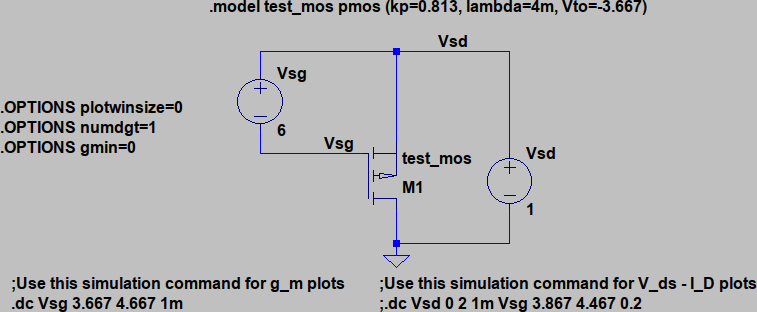
\includegraphics[width=\linewidth]{../images/ltspice_pmos_output_characteristic.png}
        \caption{LTSpice model.}
        \label{fig:ltspice_mosfet_output_characteristic}
    \end{subfigure}
    \caption{P-channel MOSFET circuit and its LTSpice model.}
\end{figure}

Do note, that the $V_{DS}$ and $V_{GS}$ are inverted and given as $V_{SD}$ and $V_{SG}$. The reason is, that the plotter in LTSpice works better with positive numbers to guess the correct scaling of the axis. Figure \ref{fig:ltspice_mosfet_output_characteristic} shows the same circuit drawn in LTSpice. The MOSFET parameters are entered using the \textbf{.model} syntax
\begin{lstlisting}[frame=single, xleftmargin=5mm, xrightmargin=5mm, columns=fullflexible, morekeywords={model, dc}, keywordstyle=\bfseries, basicstyle=\rmfamily]]
.model test_mos pmos (kp=0.813, lambda=4m, Vto=-3.667)
\end{lstlisting}
with the parameters $\kappa = \qty[per-mode=power]{0.813}{\ampere \per \square\volt}$, $\lambda = \qty[per-mode=power]{4}{\per \milli \volt}$ and $V_{th} = \qty{-3.667}{\V}$. The options \textbf{plotwinsize} and \textbf{numdgt} make sure, that LTSpice does not compress the output data and increases the floating point precision. This is important, because $I_D$ spans a large range values. Setting \textbf{gmin} to \num{0} prevents LTSpice from adding small transconductance to every pn-junction, thus changing the MOSFET model. Finally, the most important command is the \textbf{.dc} command, which instructs LTSpice to step the voltage sources $V_{SD}$ and $V_{SG}$ to evaluate $I_D$ over $V_{SD}$. The command
\begin{lstlisting}[frame=single, xleftmargin=5mm, xrightmargin=5mm, columns=fullflexible, morekeywords={model, dc}, keywordstyle=\bfseries, basicstyle=\rmfamily]]
.dc Vsd 0 2 1m Vsg 3.867 4.467 0.2
\end{lstlisting}
steps the voltage source $V_{SD}$ from $\qtyrange{0}{2}{\V}$ in steps of \qty{10}{\mV} and for each step of $V_{SD}$, steps $V_{SG}$ from \qtyrange{0.2}{0.8}{\V - V_{th}} in steps of \qty{200}{\mV}. Plotting
\begin{lstlisting}[frame=single, xleftmargin=5mm, xrightmargin=5mm, columns=fullflexible, morekeywords={model, dc}, keywordstyle=\bfseries, basicstyle=\rmfamily]]
Id(M1)
\end{lstlisting}
results in the plot shown in figure \ref{fig:ltspice_mosfet_drain_current_example}, which can be found in datasheets as the \textit{Typical Output Characteristics} plot.
To draw a line in the graph showing the point where the MOSFET enters the saturation region, denoted $I_{sat}$ in figure \ref{fig:ltspice_mosfet_drain_current_example}, as given by equation \ref{eqn:mosfet_id_large_signal}, add the following plot command to the graphing window and resecale the axis.
\begin{lstlisting}[frame=single, xleftmargin=5mm, xrightmargin=5mm, columns=fullflexible, morekeywords={model, dc}, keywordstyle=\bfseries, basicstyle=\rmfamily]]
0.5*0.813*1A/1V**2*V(vsd)**2
\end{lstlisting}
This command must be adjusted for the value of $\kappa$ and do note, that $\kappa$ is entered with units of \unit{\A \per \square\volt} to correctly display the output in \unit{\A}.

\subsection{MOSFET Transconductance}
Another interesting property to plot is the transconductance $g_m$ of the MOSFET. Again, using the same model used previously in figure \ref{fig:ltspice_mosfet_output_characteristic} and from equation \ref{eqn:mosfet_gm} we known that $g_m$ is defined as
\begin{equation}
    g_{m} = \left. \frac{\partial I_{D}}{\partial V_{GS}} \right|_{V_{DS} = const} \,. \nonumber
\end{equation}
To derive $g_m$, we need to generate values of $I_D(V_{GS})$. This can again be done by stepping $V_{GS}$
\begin{lstlisting}[frame=single, xleftmargin=5mm, xrightmargin=5mm, columns=fullflexible, morekeywords={model, dc}, keywordstyle=\bfseries, basicstyle=\rmfamily]]
.dc Vsg 3.667 4.667 1m
\end{lstlisting}
To produce a smooth plot, the the steps size of $V_{SG}$ was decreased to \qty{1}{\mV}. $V_{DS}$ is now fixed and can be set using the voltage source $V_{SD}$. The MOSFET is intentionally biased into the saturation region at $V_{DS} = \qty{-1}{\V}$ as can be seen in figure \ref{fig:ltspice_mosfet_drain_current_example}.

LTSpice is now able to numerically differentiate the data, which can be invoked by by plotting
\begin{lstlisting}[frame=single, xleftmargin=5mm, xrightmargin=5mm, columns=fullflexible, morekeywords={model, dc}, keywordstyle=\bfseries, basicstyle=\rmfamily]]
 -d(Id(M1))
\end{lstlisting}

The minus sign comes from the inverted $V_{SG} = -V_{GS}$. To plot $g_m$ over $I_D$, the formula for $g_m$ given above needs to entered manually into the \textit{Expression Editor} by right clicking the expression label on top of the graph. Finally, the x-axis must be changed to $Id(M1)$, leading to the plot in figure \ref{fig:ltspice_mosfet_gm_example}.

\begin{figure}[hb]
    \centering
    %% Creator: Matplotlib, PGF backend
%%
%% To include the figure in your LaTeX document, write
%%   \input{<filename>.pgf}
%%
%% Make sure the required packages are loaded in your preamble
%%   \usepackage{pgf}
%%
%% Also ensure that all the required font packages are loaded; for instance,
%% the lmodern package is sometimes necessary when using math font.
%%   \usepackage{lmodern}
%%
%% Figures using additional raster images can only be included by \input if
%% they are in the same directory as the main LaTeX file. For loading figures
%% from other directories you can use the `import` package
%%   \usepackage{import}
%%
%% and then include the figures with
%%   \import{<path to file>}{<filename>.pgf}
%%
%% Matplotlib used the following preamble
%%   \usepackage{siunitx}
%%   \usepackage{fontspec}
%%
\begingroup%
\makeatletter%
\begin{pgfpicture}%
\pgfpathrectangle{\pgfpointorigin}{\pgfqpoint{5.492126in}{3.394321in}}%
\pgfusepath{use as bounding box, clip}%
\begin{pgfscope}%
\pgfsetbuttcap%
\pgfsetmiterjoin%
\definecolor{currentfill}{rgb}{1.000000,1.000000,1.000000}%
\pgfsetfillcolor{currentfill}%
\pgfsetlinewidth{0.000000pt}%
\definecolor{currentstroke}{rgb}{1.000000,1.000000,1.000000}%
\pgfsetstrokecolor{currentstroke}%
\pgfsetdash{}{0pt}%
\pgfpathmoveto{\pgfqpoint{0.000000in}{0.000000in}}%
\pgfpathlineto{\pgfqpoint{5.492126in}{0.000000in}}%
\pgfpathlineto{\pgfqpoint{5.492126in}{3.394321in}}%
\pgfpathlineto{\pgfqpoint{0.000000in}{3.394321in}}%
\pgfpathlineto{\pgfqpoint{0.000000in}{0.000000in}}%
\pgfpathclose%
\pgfusepath{fill}%
\end{pgfscope}%
\begin{pgfscope}%
\pgfsetbuttcap%
\pgfsetmiterjoin%
\definecolor{currentfill}{rgb}{1.000000,1.000000,1.000000}%
\pgfsetfillcolor{currentfill}%
\pgfsetlinewidth{0.000000pt}%
\definecolor{currentstroke}{rgb}{0.000000,0.000000,0.000000}%
\pgfsetstrokecolor{currentstroke}%
\pgfsetstrokeopacity{0.000000}%
\pgfsetdash{}{0pt}%
\pgfpathmoveto{\pgfqpoint{0.602198in}{0.524170in}}%
\pgfpathlineto{\pgfqpoint{5.342126in}{0.524170in}}%
\pgfpathlineto{\pgfqpoint{5.342126in}{3.120077in}}%
\pgfpathlineto{\pgfqpoint{0.602198in}{3.120077in}}%
\pgfpathlineto{\pgfqpoint{0.602198in}{0.524170in}}%
\pgfpathclose%
\pgfusepath{fill}%
\end{pgfscope}%
\begin{pgfscope}%
\pgfpathrectangle{\pgfqpoint{0.602198in}{0.524170in}}{\pgfqpoint{4.739929in}{2.595908in}}%
\pgfusepath{clip}%
\pgfsetrectcap%
\pgfsetroundjoin%
\pgfsetlinewidth{0.803000pt}%
\definecolor{currentstroke}{rgb}{0.450000,0.450000,0.450000}%
\pgfsetstrokecolor{currentstroke}%
\pgfsetdash{}{0pt}%
\pgfpathmoveto{\pgfqpoint{5.040880in}{0.524170in}}%
\pgfpathlineto{\pgfqpoint{5.040880in}{3.120077in}}%
\pgfusepath{stroke}%
\end{pgfscope}%
\begin{pgfscope}%
\pgfsetbuttcap%
\pgfsetroundjoin%
\definecolor{currentfill}{rgb}{0.000000,0.000000,0.000000}%
\pgfsetfillcolor{currentfill}%
\pgfsetlinewidth{0.803000pt}%
\definecolor{currentstroke}{rgb}{0.000000,0.000000,0.000000}%
\pgfsetstrokecolor{currentstroke}%
\pgfsetdash{}{0pt}%
\pgfsys@defobject{currentmarker}{\pgfqpoint{0.000000in}{-0.048611in}}{\pgfqpoint{0.000000in}{0.000000in}}{%
\pgfpathmoveto{\pgfqpoint{0.000000in}{0.000000in}}%
\pgfpathlineto{\pgfqpoint{0.000000in}{-0.048611in}}%
\pgfusepath{stroke,fill}%
}%
\begin{pgfscope}%
\pgfsys@transformshift{5.040880in}{0.524170in}%
\pgfsys@useobject{currentmarker}{}%
\end{pgfscope}%
\end{pgfscope}%
\begin{pgfscope}%
\definecolor{textcolor}{rgb}{0.000000,0.000000,0.000000}%
\pgfsetstrokecolor{textcolor}%
\pgfsetfillcolor{textcolor}%
\pgftext[x=5.040880in,y=0.426948in,,top]{\color{textcolor}\rmfamily\fontsize{8.000000}{9.600000}\selectfont \(\displaystyle {\ensuremath{-}0.40}\)}%
\end{pgfscope}%
\begin{pgfscope}%
\pgfpathrectangle{\pgfqpoint{0.602198in}{0.524170in}}{\pgfqpoint{4.739929in}{2.595908in}}%
\pgfusepath{clip}%
\pgfsetrectcap%
\pgfsetroundjoin%
\pgfsetlinewidth{0.803000pt}%
\definecolor{currentstroke}{rgb}{0.450000,0.450000,0.450000}%
\pgfsetstrokecolor{currentstroke}%
\pgfsetdash{}{0pt}%
\pgfpathmoveto{\pgfqpoint{4.512976in}{0.524170in}}%
\pgfpathlineto{\pgfqpoint{4.512976in}{3.120077in}}%
\pgfusepath{stroke}%
\end{pgfscope}%
\begin{pgfscope}%
\pgfsetbuttcap%
\pgfsetroundjoin%
\definecolor{currentfill}{rgb}{0.000000,0.000000,0.000000}%
\pgfsetfillcolor{currentfill}%
\pgfsetlinewidth{0.803000pt}%
\definecolor{currentstroke}{rgb}{0.000000,0.000000,0.000000}%
\pgfsetstrokecolor{currentstroke}%
\pgfsetdash{}{0pt}%
\pgfsys@defobject{currentmarker}{\pgfqpoint{0.000000in}{-0.048611in}}{\pgfqpoint{0.000000in}{0.000000in}}{%
\pgfpathmoveto{\pgfqpoint{0.000000in}{0.000000in}}%
\pgfpathlineto{\pgfqpoint{0.000000in}{-0.048611in}}%
\pgfusepath{stroke,fill}%
}%
\begin{pgfscope}%
\pgfsys@transformshift{4.512976in}{0.524170in}%
\pgfsys@useobject{currentmarker}{}%
\end{pgfscope}%
\end{pgfscope}%
\begin{pgfscope}%
\definecolor{textcolor}{rgb}{0.000000,0.000000,0.000000}%
\pgfsetstrokecolor{textcolor}%
\pgfsetfillcolor{textcolor}%
\pgftext[x=4.512976in,y=0.426948in,,top]{\color{textcolor}\rmfamily\fontsize{8.000000}{9.600000}\selectfont \(\displaystyle {\ensuremath{-}0.35}\)}%
\end{pgfscope}%
\begin{pgfscope}%
\pgfpathrectangle{\pgfqpoint{0.602198in}{0.524170in}}{\pgfqpoint{4.739929in}{2.595908in}}%
\pgfusepath{clip}%
\pgfsetrectcap%
\pgfsetroundjoin%
\pgfsetlinewidth{0.803000pt}%
\definecolor{currentstroke}{rgb}{0.450000,0.450000,0.450000}%
\pgfsetstrokecolor{currentstroke}%
\pgfsetdash{}{0pt}%
\pgfpathmoveto{\pgfqpoint{3.985072in}{0.524170in}}%
\pgfpathlineto{\pgfqpoint{3.985072in}{3.120077in}}%
\pgfusepath{stroke}%
\end{pgfscope}%
\begin{pgfscope}%
\pgfsetbuttcap%
\pgfsetroundjoin%
\definecolor{currentfill}{rgb}{0.000000,0.000000,0.000000}%
\pgfsetfillcolor{currentfill}%
\pgfsetlinewidth{0.803000pt}%
\definecolor{currentstroke}{rgb}{0.000000,0.000000,0.000000}%
\pgfsetstrokecolor{currentstroke}%
\pgfsetdash{}{0pt}%
\pgfsys@defobject{currentmarker}{\pgfqpoint{0.000000in}{-0.048611in}}{\pgfqpoint{0.000000in}{0.000000in}}{%
\pgfpathmoveto{\pgfqpoint{0.000000in}{0.000000in}}%
\pgfpathlineto{\pgfqpoint{0.000000in}{-0.048611in}}%
\pgfusepath{stroke,fill}%
}%
\begin{pgfscope}%
\pgfsys@transformshift{3.985072in}{0.524170in}%
\pgfsys@useobject{currentmarker}{}%
\end{pgfscope}%
\end{pgfscope}%
\begin{pgfscope}%
\definecolor{textcolor}{rgb}{0.000000,0.000000,0.000000}%
\pgfsetstrokecolor{textcolor}%
\pgfsetfillcolor{textcolor}%
\pgftext[x=3.985072in,y=0.426948in,,top]{\color{textcolor}\rmfamily\fontsize{8.000000}{9.600000}\selectfont \(\displaystyle {\ensuremath{-}0.30}\)}%
\end{pgfscope}%
\begin{pgfscope}%
\pgfpathrectangle{\pgfqpoint{0.602198in}{0.524170in}}{\pgfqpoint{4.739929in}{2.595908in}}%
\pgfusepath{clip}%
\pgfsetrectcap%
\pgfsetroundjoin%
\pgfsetlinewidth{0.803000pt}%
\definecolor{currentstroke}{rgb}{0.450000,0.450000,0.450000}%
\pgfsetstrokecolor{currentstroke}%
\pgfsetdash{}{0pt}%
\pgfpathmoveto{\pgfqpoint{3.457168in}{0.524170in}}%
\pgfpathlineto{\pgfqpoint{3.457168in}{3.120077in}}%
\pgfusepath{stroke}%
\end{pgfscope}%
\begin{pgfscope}%
\pgfsetbuttcap%
\pgfsetroundjoin%
\definecolor{currentfill}{rgb}{0.000000,0.000000,0.000000}%
\pgfsetfillcolor{currentfill}%
\pgfsetlinewidth{0.803000pt}%
\definecolor{currentstroke}{rgb}{0.000000,0.000000,0.000000}%
\pgfsetstrokecolor{currentstroke}%
\pgfsetdash{}{0pt}%
\pgfsys@defobject{currentmarker}{\pgfqpoint{0.000000in}{-0.048611in}}{\pgfqpoint{0.000000in}{0.000000in}}{%
\pgfpathmoveto{\pgfqpoint{0.000000in}{0.000000in}}%
\pgfpathlineto{\pgfqpoint{0.000000in}{-0.048611in}}%
\pgfusepath{stroke,fill}%
}%
\begin{pgfscope}%
\pgfsys@transformshift{3.457168in}{0.524170in}%
\pgfsys@useobject{currentmarker}{}%
\end{pgfscope}%
\end{pgfscope}%
\begin{pgfscope}%
\definecolor{textcolor}{rgb}{0.000000,0.000000,0.000000}%
\pgfsetstrokecolor{textcolor}%
\pgfsetfillcolor{textcolor}%
\pgftext[x=3.457168in,y=0.426948in,,top]{\color{textcolor}\rmfamily\fontsize{8.000000}{9.600000}\selectfont \(\displaystyle {\ensuremath{-}0.25}\)}%
\end{pgfscope}%
\begin{pgfscope}%
\pgfpathrectangle{\pgfqpoint{0.602198in}{0.524170in}}{\pgfqpoint{4.739929in}{2.595908in}}%
\pgfusepath{clip}%
\pgfsetrectcap%
\pgfsetroundjoin%
\pgfsetlinewidth{0.803000pt}%
\definecolor{currentstroke}{rgb}{0.450000,0.450000,0.450000}%
\pgfsetstrokecolor{currentstroke}%
\pgfsetdash{}{0pt}%
\pgfpathmoveto{\pgfqpoint{2.929264in}{0.524170in}}%
\pgfpathlineto{\pgfqpoint{2.929264in}{3.120077in}}%
\pgfusepath{stroke}%
\end{pgfscope}%
\begin{pgfscope}%
\pgfsetbuttcap%
\pgfsetroundjoin%
\definecolor{currentfill}{rgb}{0.000000,0.000000,0.000000}%
\pgfsetfillcolor{currentfill}%
\pgfsetlinewidth{0.803000pt}%
\definecolor{currentstroke}{rgb}{0.000000,0.000000,0.000000}%
\pgfsetstrokecolor{currentstroke}%
\pgfsetdash{}{0pt}%
\pgfsys@defobject{currentmarker}{\pgfqpoint{0.000000in}{-0.048611in}}{\pgfqpoint{0.000000in}{0.000000in}}{%
\pgfpathmoveto{\pgfqpoint{0.000000in}{0.000000in}}%
\pgfpathlineto{\pgfqpoint{0.000000in}{-0.048611in}}%
\pgfusepath{stroke,fill}%
}%
\begin{pgfscope}%
\pgfsys@transformshift{2.929264in}{0.524170in}%
\pgfsys@useobject{currentmarker}{}%
\end{pgfscope}%
\end{pgfscope}%
\begin{pgfscope}%
\definecolor{textcolor}{rgb}{0.000000,0.000000,0.000000}%
\pgfsetstrokecolor{textcolor}%
\pgfsetfillcolor{textcolor}%
\pgftext[x=2.929264in,y=0.426948in,,top]{\color{textcolor}\rmfamily\fontsize{8.000000}{9.600000}\selectfont \(\displaystyle {\ensuremath{-}0.20}\)}%
\end{pgfscope}%
\begin{pgfscope}%
\pgfpathrectangle{\pgfqpoint{0.602198in}{0.524170in}}{\pgfqpoint{4.739929in}{2.595908in}}%
\pgfusepath{clip}%
\pgfsetrectcap%
\pgfsetroundjoin%
\pgfsetlinewidth{0.803000pt}%
\definecolor{currentstroke}{rgb}{0.450000,0.450000,0.450000}%
\pgfsetstrokecolor{currentstroke}%
\pgfsetdash{}{0pt}%
\pgfpathmoveto{\pgfqpoint{2.401361in}{0.524170in}}%
\pgfpathlineto{\pgfqpoint{2.401361in}{3.120077in}}%
\pgfusepath{stroke}%
\end{pgfscope}%
\begin{pgfscope}%
\pgfsetbuttcap%
\pgfsetroundjoin%
\definecolor{currentfill}{rgb}{0.000000,0.000000,0.000000}%
\pgfsetfillcolor{currentfill}%
\pgfsetlinewidth{0.803000pt}%
\definecolor{currentstroke}{rgb}{0.000000,0.000000,0.000000}%
\pgfsetstrokecolor{currentstroke}%
\pgfsetdash{}{0pt}%
\pgfsys@defobject{currentmarker}{\pgfqpoint{0.000000in}{-0.048611in}}{\pgfqpoint{0.000000in}{0.000000in}}{%
\pgfpathmoveto{\pgfqpoint{0.000000in}{0.000000in}}%
\pgfpathlineto{\pgfqpoint{0.000000in}{-0.048611in}}%
\pgfusepath{stroke,fill}%
}%
\begin{pgfscope}%
\pgfsys@transformshift{2.401361in}{0.524170in}%
\pgfsys@useobject{currentmarker}{}%
\end{pgfscope}%
\end{pgfscope}%
\begin{pgfscope}%
\definecolor{textcolor}{rgb}{0.000000,0.000000,0.000000}%
\pgfsetstrokecolor{textcolor}%
\pgfsetfillcolor{textcolor}%
\pgftext[x=2.401361in,y=0.426948in,,top]{\color{textcolor}\rmfamily\fontsize{8.000000}{9.600000}\selectfont \(\displaystyle {\ensuremath{-}0.15}\)}%
\end{pgfscope}%
\begin{pgfscope}%
\pgfpathrectangle{\pgfqpoint{0.602198in}{0.524170in}}{\pgfqpoint{4.739929in}{2.595908in}}%
\pgfusepath{clip}%
\pgfsetrectcap%
\pgfsetroundjoin%
\pgfsetlinewidth{0.803000pt}%
\definecolor{currentstroke}{rgb}{0.450000,0.450000,0.450000}%
\pgfsetstrokecolor{currentstroke}%
\pgfsetdash{}{0pt}%
\pgfpathmoveto{\pgfqpoint{1.873457in}{0.524170in}}%
\pgfpathlineto{\pgfqpoint{1.873457in}{3.120077in}}%
\pgfusepath{stroke}%
\end{pgfscope}%
\begin{pgfscope}%
\pgfsetbuttcap%
\pgfsetroundjoin%
\definecolor{currentfill}{rgb}{0.000000,0.000000,0.000000}%
\pgfsetfillcolor{currentfill}%
\pgfsetlinewidth{0.803000pt}%
\definecolor{currentstroke}{rgb}{0.000000,0.000000,0.000000}%
\pgfsetstrokecolor{currentstroke}%
\pgfsetdash{}{0pt}%
\pgfsys@defobject{currentmarker}{\pgfqpoint{0.000000in}{-0.048611in}}{\pgfqpoint{0.000000in}{0.000000in}}{%
\pgfpathmoveto{\pgfqpoint{0.000000in}{0.000000in}}%
\pgfpathlineto{\pgfqpoint{0.000000in}{-0.048611in}}%
\pgfusepath{stroke,fill}%
}%
\begin{pgfscope}%
\pgfsys@transformshift{1.873457in}{0.524170in}%
\pgfsys@useobject{currentmarker}{}%
\end{pgfscope}%
\end{pgfscope}%
\begin{pgfscope}%
\definecolor{textcolor}{rgb}{0.000000,0.000000,0.000000}%
\pgfsetstrokecolor{textcolor}%
\pgfsetfillcolor{textcolor}%
\pgftext[x=1.873457in,y=0.426948in,,top]{\color{textcolor}\rmfamily\fontsize{8.000000}{9.600000}\selectfont \(\displaystyle {\ensuremath{-}0.10}\)}%
\end{pgfscope}%
\begin{pgfscope}%
\pgfpathrectangle{\pgfqpoint{0.602198in}{0.524170in}}{\pgfqpoint{4.739929in}{2.595908in}}%
\pgfusepath{clip}%
\pgfsetrectcap%
\pgfsetroundjoin%
\pgfsetlinewidth{0.803000pt}%
\definecolor{currentstroke}{rgb}{0.450000,0.450000,0.450000}%
\pgfsetstrokecolor{currentstroke}%
\pgfsetdash{}{0pt}%
\pgfpathmoveto{\pgfqpoint{1.345553in}{0.524170in}}%
\pgfpathlineto{\pgfqpoint{1.345553in}{3.120077in}}%
\pgfusepath{stroke}%
\end{pgfscope}%
\begin{pgfscope}%
\pgfsetbuttcap%
\pgfsetroundjoin%
\definecolor{currentfill}{rgb}{0.000000,0.000000,0.000000}%
\pgfsetfillcolor{currentfill}%
\pgfsetlinewidth{0.803000pt}%
\definecolor{currentstroke}{rgb}{0.000000,0.000000,0.000000}%
\pgfsetstrokecolor{currentstroke}%
\pgfsetdash{}{0pt}%
\pgfsys@defobject{currentmarker}{\pgfqpoint{0.000000in}{-0.048611in}}{\pgfqpoint{0.000000in}{0.000000in}}{%
\pgfpathmoveto{\pgfqpoint{0.000000in}{0.000000in}}%
\pgfpathlineto{\pgfqpoint{0.000000in}{-0.048611in}}%
\pgfusepath{stroke,fill}%
}%
\begin{pgfscope}%
\pgfsys@transformshift{1.345553in}{0.524170in}%
\pgfsys@useobject{currentmarker}{}%
\end{pgfscope}%
\end{pgfscope}%
\begin{pgfscope}%
\definecolor{textcolor}{rgb}{0.000000,0.000000,0.000000}%
\pgfsetstrokecolor{textcolor}%
\pgfsetfillcolor{textcolor}%
\pgftext[x=1.345553in,y=0.426948in,,top]{\color{textcolor}\rmfamily\fontsize{8.000000}{9.600000}\selectfont \(\displaystyle {\ensuremath{-}0.05}\)}%
\end{pgfscope}%
\begin{pgfscope}%
\pgfpathrectangle{\pgfqpoint{0.602198in}{0.524170in}}{\pgfqpoint{4.739929in}{2.595908in}}%
\pgfusepath{clip}%
\pgfsetrectcap%
\pgfsetroundjoin%
\pgfsetlinewidth{0.803000pt}%
\definecolor{currentstroke}{rgb}{0.450000,0.450000,0.450000}%
\pgfsetstrokecolor{currentstroke}%
\pgfsetdash{}{0pt}%
\pgfpathmoveto{\pgfqpoint{0.817649in}{0.524170in}}%
\pgfpathlineto{\pgfqpoint{0.817649in}{3.120077in}}%
\pgfusepath{stroke}%
\end{pgfscope}%
\begin{pgfscope}%
\pgfsetbuttcap%
\pgfsetroundjoin%
\definecolor{currentfill}{rgb}{0.000000,0.000000,0.000000}%
\pgfsetfillcolor{currentfill}%
\pgfsetlinewidth{0.803000pt}%
\definecolor{currentstroke}{rgb}{0.000000,0.000000,0.000000}%
\pgfsetstrokecolor{currentstroke}%
\pgfsetdash{}{0pt}%
\pgfsys@defobject{currentmarker}{\pgfqpoint{0.000000in}{-0.048611in}}{\pgfqpoint{0.000000in}{0.000000in}}{%
\pgfpathmoveto{\pgfqpoint{0.000000in}{0.000000in}}%
\pgfpathlineto{\pgfqpoint{0.000000in}{-0.048611in}}%
\pgfusepath{stroke,fill}%
}%
\begin{pgfscope}%
\pgfsys@transformshift{0.817649in}{0.524170in}%
\pgfsys@useobject{currentmarker}{}%
\end{pgfscope}%
\end{pgfscope}%
\begin{pgfscope}%
\definecolor{textcolor}{rgb}{0.000000,0.000000,0.000000}%
\pgfsetstrokecolor{textcolor}%
\pgfsetfillcolor{textcolor}%
\pgftext[x=0.817649in,y=0.426948in,,top]{\color{textcolor}\rmfamily\fontsize{8.000000}{9.600000}\selectfont \(\displaystyle {0.00}\)}%
\end{pgfscope}%
\begin{pgfscope}%
\definecolor{textcolor}{rgb}{0.000000,0.000000,0.000000}%
\pgfsetstrokecolor{textcolor}%
\pgfsetfillcolor{textcolor}%
\pgftext[x=2.972162in,y=0.272725in,,top]{\color{textcolor}\rmfamily\fontsize{10.000000}{12.000000}\selectfont Drain Current \(\displaystyle I_{D}\) in \unit{\A}}%
\end{pgfscope}%
\begin{pgfscope}%
\pgfpathrectangle{\pgfqpoint{0.602198in}{0.524170in}}{\pgfqpoint{4.739929in}{2.595908in}}%
\pgfusepath{clip}%
\pgfsetrectcap%
\pgfsetroundjoin%
\pgfsetlinewidth{0.803000pt}%
\definecolor{currentstroke}{rgb}{0.450000,0.450000,0.450000}%
\pgfsetstrokecolor{currentstroke}%
\pgfsetdash{}{0pt}%
\pgfpathmoveto{\pgfqpoint{0.602198in}{0.640984in}}%
\pgfpathlineto{\pgfqpoint{5.342126in}{0.640984in}}%
\pgfusepath{stroke}%
\end{pgfscope}%
\begin{pgfscope}%
\pgfsetbuttcap%
\pgfsetroundjoin%
\definecolor{currentfill}{rgb}{0.000000,0.000000,0.000000}%
\pgfsetfillcolor{currentfill}%
\pgfsetlinewidth{0.803000pt}%
\definecolor{currentstroke}{rgb}{0.000000,0.000000,0.000000}%
\pgfsetstrokecolor{currentstroke}%
\pgfsetdash{}{0pt}%
\pgfsys@defobject{currentmarker}{\pgfqpoint{-0.048611in}{0.000000in}}{\pgfqpoint{-0.000000in}{0.000000in}}{%
\pgfpathmoveto{\pgfqpoint{-0.000000in}{0.000000in}}%
\pgfpathlineto{\pgfqpoint{-0.048611in}{0.000000in}}%
\pgfusepath{stroke,fill}%
}%
\begin{pgfscope}%
\pgfsys@transformshift{0.602198in}{0.640984in}%
\pgfsys@useobject{currentmarker}{}%
\end{pgfscope}%
\end{pgfscope}%
\begin{pgfscope}%
\definecolor{textcolor}{rgb}{0.000000,0.000000,0.000000}%
\pgfsetstrokecolor{textcolor}%
\pgfsetfillcolor{textcolor}%
\pgftext[x=0.445947in, y=0.602429in, left, base]{\color{textcolor}\rmfamily\fontsize{8.000000}{9.600000}\selectfont \(\displaystyle {0}\)}%
\end{pgfscope}%
\begin{pgfscope}%
\pgfpathrectangle{\pgfqpoint{0.602198in}{0.524170in}}{\pgfqpoint{4.739929in}{2.595908in}}%
\pgfusepath{clip}%
\pgfsetrectcap%
\pgfsetroundjoin%
\pgfsetlinewidth{0.803000pt}%
\definecolor{currentstroke}{rgb}{0.450000,0.450000,0.450000}%
\pgfsetstrokecolor{currentstroke}%
\pgfsetdash{}{0pt}%
\pgfpathmoveto{\pgfqpoint{0.602198in}{0.930390in}}%
\pgfpathlineto{\pgfqpoint{5.342126in}{0.930390in}}%
\pgfusepath{stroke}%
\end{pgfscope}%
\begin{pgfscope}%
\pgfsetbuttcap%
\pgfsetroundjoin%
\definecolor{currentfill}{rgb}{0.000000,0.000000,0.000000}%
\pgfsetfillcolor{currentfill}%
\pgfsetlinewidth{0.803000pt}%
\definecolor{currentstroke}{rgb}{0.000000,0.000000,0.000000}%
\pgfsetstrokecolor{currentstroke}%
\pgfsetdash{}{0pt}%
\pgfsys@defobject{currentmarker}{\pgfqpoint{-0.048611in}{0.000000in}}{\pgfqpoint{-0.000000in}{0.000000in}}{%
\pgfpathmoveto{\pgfqpoint{-0.000000in}{0.000000in}}%
\pgfpathlineto{\pgfqpoint{-0.048611in}{0.000000in}}%
\pgfusepath{stroke,fill}%
}%
\begin{pgfscope}%
\pgfsys@transformshift{0.602198in}{0.930390in}%
\pgfsys@useobject{currentmarker}{}%
\end{pgfscope}%
\end{pgfscope}%
\begin{pgfscope}%
\definecolor{textcolor}{rgb}{0.000000,0.000000,0.000000}%
\pgfsetstrokecolor{textcolor}%
\pgfsetfillcolor{textcolor}%
\pgftext[x=0.327890in, y=0.891834in, left, base]{\color{textcolor}\rmfamily\fontsize{8.000000}{9.600000}\selectfont \(\displaystyle {100}\)}%
\end{pgfscope}%
\begin{pgfscope}%
\pgfpathrectangle{\pgfqpoint{0.602198in}{0.524170in}}{\pgfqpoint{4.739929in}{2.595908in}}%
\pgfusepath{clip}%
\pgfsetrectcap%
\pgfsetroundjoin%
\pgfsetlinewidth{0.803000pt}%
\definecolor{currentstroke}{rgb}{0.450000,0.450000,0.450000}%
\pgfsetstrokecolor{currentstroke}%
\pgfsetdash{}{0pt}%
\pgfpathmoveto{\pgfqpoint{0.602198in}{1.219795in}}%
\pgfpathlineto{\pgfqpoint{5.342126in}{1.219795in}}%
\pgfusepath{stroke}%
\end{pgfscope}%
\begin{pgfscope}%
\pgfsetbuttcap%
\pgfsetroundjoin%
\definecolor{currentfill}{rgb}{0.000000,0.000000,0.000000}%
\pgfsetfillcolor{currentfill}%
\pgfsetlinewidth{0.803000pt}%
\definecolor{currentstroke}{rgb}{0.000000,0.000000,0.000000}%
\pgfsetstrokecolor{currentstroke}%
\pgfsetdash{}{0pt}%
\pgfsys@defobject{currentmarker}{\pgfqpoint{-0.048611in}{0.000000in}}{\pgfqpoint{-0.000000in}{0.000000in}}{%
\pgfpathmoveto{\pgfqpoint{-0.000000in}{0.000000in}}%
\pgfpathlineto{\pgfqpoint{-0.048611in}{0.000000in}}%
\pgfusepath{stroke,fill}%
}%
\begin{pgfscope}%
\pgfsys@transformshift{0.602198in}{1.219795in}%
\pgfsys@useobject{currentmarker}{}%
\end{pgfscope}%
\end{pgfscope}%
\begin{pgfscope}%
\definecolor{textcolor}{rgb}{0.000000,0.000000,0.000000}%
\pgfsetstrokecolor{textcolor}%
\pgfsetfillcolor{textcolor}%
\pgftext[x=0.327890in, y=1.181240in, left, base]{\color{textcolor}\rmfamily\fontsize{8.000000}{9.600000}\selectfont \(\displaystyle {200}\)}%
\end{pgfscope}%
\begin{pgfscope}%
\pgfpathrectangle{\pgfqpoint{0.602198in}{0.524170in}}{\pgfqpoint{4.739929in}{2.595908in}}%
\pgfusepath{clip}%
\pgfsetrectcap%
\pgfsetroundjoin%
\pgfsetlinewidth{0.803000pt}%
\definecolor{currentstroke}{rgb}{0.450000,0.450000,0.450000}%
\pgfsetstrokecolor{currentstroke}%
\pgfsetdash{}{0pt}%
\pgfpathmoveto{\pgfqpoint{0.602198in}{1.509201in}}%
\pgfpathlineto{\pgfqpoint{5.342126in}{1.509201in}}%
\pgfusepath{stroke}%
\end{pgfscope}%
\begin{pgfscope}%
\pgfsetbuttcap%
\pgfsetroundjoin%
\definecolor{currentfill}{rgb}{0.000000,0.000000,0.000000}%
\pgfsetfillcolor{currentfill}%
\pgfsetlinewidth{0.803000pt}%
\definecolor{currentstroke}{rgb}{0.000000,0.000000,0.000000}%
\pgfsetstrokecolor{currentstroke}%
\pgfsetdash{}{0pt}%
\pgfsys@defobject{currentmarker}{\pgfqpoint{-0.048611in}{0.000000in}}{\pgfqpoint{-0.000000in}{0.000000in}}{%
\pgfpathmoveto{\pgfqpoint{-0.000000in}{0.000000in}}%
\pgfpathlineto{\pgfqpoint{-0.048611in}{0.000000in}}%
\pgfusepath{stroke,fill}%
}%
\begin{pgfscope}%
\pgfsys@transformshift{0.602198in}{1.509201in}%
\pgfsys@useobject{currentmarker}{}%
\end{pgfscope}%
\end{pgfscope}%
\begin{pgfscope}%
\definecolor{textcolor}{rgb}{0.000000,0.000000,0.000000}%
\pgfsetstrokecolor{textcolor}%
\pgfsetfillcolor{textcolor}%
\pgftext[x=0.327890in, y=1.470645in, left, base]{\color{textcolor}\rmfamily\fontsize{8.000000}{9.600000}\selectfont \(\displaystyle {300}\)}%
\end{pgfscope}%
\begin{pgfscope}%
\pgfpathrectangle{\pgfqpoint{0.602198in}{0.524170in}}{\pgfqpoint{4.739929in}{2.595908in}}%
\pgfusepath{clip}%
\pgfsetrectcap%
\pgfsetroundjoin%
\pgfsetlinewidth{0.803000pt}%
\definecolor{currentstroke}{rgb}{0.450000,0.450000,0.450000}%
\pgfsetstrokecolor{currentstroke}%
\pgfsetdash{}{0pt}%
\pgfpathmoveto{\pgfqpoint{0.602198in}{1.798607in}}%
\pgfpathlineto{\pgfqpoint{5.342126in}{1.798607in}}%
\pgfusepath{stroke}%
\end{pgfscope}%
\begin{pgfscope}%
\pgfsetbuttcap%
\pgfsetroundjoin%
\definecolor{currentfill}{rgb}{0.000000,0.000000,0.000000}%
\pgfsetfillcolor{currentfill}%
\pgfsetlinewidth{0.803000pt}%
\definecolor{currentstroke}{rgb}{0.000000,0.000000,0.000000}%
\pgfsetstrokecolor{currentstroke}%
\pgfsetdash{}{0pt}%
\pgfsys@defobject{currentmarker}{\pgfqpoint{-0.048611in}{0.000000in}}{\pgfqpoint{-0.000000in}{0.000000in}}{%
\pgfpathmoveto{\pgfqpoint{-0.000000in}{0.000000in}}%
\pgfpathlineto{\pgfqpoint{-0.048611in}{0.000000in}}%
\pgfusepath{stroke,fill}%
}%
\begin{pgfscope}%
\pgfsys@transformshift{0.602198in}{1.798607in}%
\pgfsys@useobject{currentmarker}{}%
\end{pgfscope}%
\end{pgfscope}%
\begin{pgfscope}%
\definecolor{textcolor}{rgb}{0.000000,0.000000,0.000000}%
\pgfsetstrokecolor{textcolor}%
\pgfsetfillcolor{textcolor}%
\pgftext[x=0.327890in, y=1.760051in, left, base]{\color{textcolor}\rmfamily\fontsize{8.000000}{9.600000}\selectfont \(\displaystyle {400}\)}%
\end{pgfscope}%
\begin{pgfscope}%
\pgfpathrectangle{\pgfqpoint{0.602198in}{0.524170in}}{\pgfqpoint{4.739929in}{2.595908in}}%
\pgfusepath{clip}%
\pgfsetrectcap%
\pgfsetroundjoin%
\pgfsetlinewidth{0.803000pt}%
\definecolor{currentstroke}{rgb}{0.450000,0.450000,0.450000}%
\pgfsetstrokecolor{currentstroke}%
\pgfsetdash{}{0pt}%
\pgfpathmoveto{\pgfqpoint{0.602198in}{2.088012in}}%
\pgfpathlineto{\pgfqpoint{5.342126in}{2.088012in}}%
\pgfusepath{stroke}%
\end{pgfscope}%
\begin{pgfscope}%
\pgfsetbuttcap%
\pgfsetroundjoin%
\definecolor{currentfill}{rgb}{0.000000,0.000000,0.000000}%
\pgfsetfillcolor{currentfill}%
\pgfsetlinewidth{0.803000pt}%
\definecolor{currentstroke}{rgb}{0.000000,0.000000,0.000000}%
\pgfsetstrokecolor{currentstroke}%
\pgfsetdash{}{0pt}%
\pgfsys@defobject{currentmarker}{\pgfqpoint{-0.048611in}{0.000000in}}{\pgfqpoint{-0.000000in}{0.000000in}}{%
\pgfpathmoveto{\pgfqpoint{-0.000000in}{0.000000in}}%
\pgfpathlineto{\pgfqpoint{-0.048611in}{0.000000in}}%
\pgfusepath{stroke,fill}%
}%
\begin{pgfscope}%
\pgfsys@transformshift{0.602198in}{2.088012in}%
\pgfsys@useobject{currentmarker}{}%
\end{pgfscope}%
\end{pgfscope}%
\begin{pgfscope}%
\definecolor{textcolor}{rgb}{0.000000,0.000000,0.000000}%
\pgfsetstrokecolor{textcolor}%
\pgfsetfillcolor{textcolor}%
\pgftext[x=0.327890in, y=2.049456in, left, base]{\color{textcolor}\rmfamily\fontsize{8.000000}{9.600000}\selectfont \(\displaystyle {500}\)}%
\end{pgfscope}%
\begin{pgfscope}%
\pgfpathrectangle{\pgfqpoint{0.602198in}{0.524170in}}{\pgfqpoint{4.739929in}{2.595908in}}%
\pgfusepath{clip}%
\pgfsetrectcap%
\pgfsetroundjoin%
\pgfsetlinewidth{0.803000pt}%
\definecolor{currentstroke}{rgb}{0.450000,0.450000,0.450000}%
\pgfsetstrokecolor{currentstroke}%
\pgfsetdash{}{0pt}%
\pgfpathmoveto{\pgfqpoint{0.602198in}{2.377418in}}%
\pgfpathlineto{\pgfqpoint{5.342126in}{2.377418in}}%
\pgfusepath{stroke}%
\end{pgfscope}%
\begin{pgfscope}%
\pgfsetbuttcap%
\pgfsetroundjoin%
\definecolor{currentfill}{rgb}{0.000000,0.000000,0.000000}%
\pgfsetfillcolor{currentfill}%
\pgfsetlinewidth{0.803000pt}%
\definecolor{currentstroke}{rgb}{0.000000,0.000000,0.000000}%
\pgfsetstrokecolor{currentstroke}%
\pgfsetdash{}{0pt}%
\pgfsys@defobject{currentmarker}{\pgfqpoint{-0.048611in}{0.000000in}}{\pgfqpoint{-0.000000in}{0.000000in}}{%
\pgfpathmoveto{\pgfqpoint{-0.000000in}{0.000000in}}%
\pgfpathlineto{\pgfqpoint{-0.048611in}{0.000000in}}%
\pgfusepath{stroke,fill}%
}%
\begin{pgfscope}%
\pgfsys@transformshift{0.602198in}{2.377418in}%
\pgfsys@useobject{currentmarker}{}%
\end{pgfscope}%
\end{pgfscope}%
\begin{pgfscope}%
\definecolor{textcolor}{rgb}{0.000000,0.000000,0.000000}%
\pgfsetstrokecolor{textcolor}%
\pgfsetfillcolor{textcolor}%
\pgftext[x=0.327890in, y=2.338862in, left, base]{\color{textcolor}\rmfamily\fontsize{8.000000}{9.600000}\selectfont \(\displaystyle {600}\)}%
\end{pgfscope}%
\begin{pgfscope}%
\pgfpathrectangle{\pgfqpoint{0.602198in}{0.524170in}}{\pgfqpoint{4.739929in}{2.595908in}}%
\pgfusepath{clip}%
\pgfsetrectcap%
\pgfsetroundjoin%
\pgfsetlinewidth{0.803000pt}%
\definecolor{currentstroke}{rgb}{0.450000,0.450000,0.450000}%
\pgfsetstrokecolor{currentstroke}%
\pgfsetdash{}{0pt}%
\pgfpathmoveto{\pgfqpoint{0.602198in}{2.666823in}}%
\pgfpathlineto{\pgfqpoint{5.342126in}{2.666823in}}%
\pgfusepath{stroke}%
\end{pgfscope}%
\begin{pgfscope}%
\pgfsetbuttcap%
\pgfsetroundjoin%
\definecolor{currentfill}{rgb}{0.000000,0.000000,0.000000}%
\pgfsetfillcolor{currentfill}%
\pgfsetlinewidth{0.803000pt}%
\definecolor{currentstroke}{rgb}{0.000000,0.000000,0.000000}%
\pgfsetstrokecolor{currentstroke}%
\pgfsetdash{}{0pt}%
\pgfsys@defobject{currentmarker}{\pgfqpoint{-0.048611in}{0.000000in}}{\pgfqpoint{-0.000000in}{0.000000in}}{%
\pgfpathmoveto{\pgfqpoint{-0.000000in}{0.000000in}}%
\pgfpathlineto{\pgfqpoint{-0.048611in}{0.000000in}}%
\pgfusepath{stroke,fill}%
}%
\begin{pgfscope}%
\pgfsys@transformshift{0.602198in}{2.666823in}%
\pgfsys@useobject{currentmarker}{}%
\end{pgfscope}%
\end{pgfscope}%
\begin{pgfscope}%
\definecolor{textcolor}{rgb}{0.000000,0.000000,0.000000}%
\pgfsetstrokecolor{textcolor}%
\pgfsetfillcolor{textcolor}%
\pgftext[x=0.327890in, y=2.628268in, left, base]{\color{textcolor}\rmfamily\fontsize{8.000000}{9.600000}\selectfont \(\displaystyle {700}\)}%
\end{pgfscope}%
\begin{pgfscope}%
\pgfpathrectangle{\pgfqpoint{0.602198in}{0.524170in}}{\pgfqpoint{4.739929in}{2.595908in}}%
\pgfusepath{clip}%
\pgfsetrectcap%
\pgfsetroundjoin%
\pgfsetlinewidth{0.803000pt}%
\definecolor{currentstroke}{rgb}{0.450000,0.450000,0.450000}%
\pgfsetstrokecolor{currentstroke}%
\pgfsetdash{}{0pt}%
\pgfpathmoveto{\pgfqpoint{0.602198in}{2.956229in}}%
\pgfpathlineto{\pgfqpoint{5.342126in}{2.956229in}}%
\pgfusepath{stroke}%
\end{pgfscope}%
\begin{pgfscope}%
\pgfsetbuttcap%
\pgfsetroundjoin%
\definecolor{currentfill}{rgb}{0.000000,0.000000,0.000000}%
\pgfsetfillcolor{currentfill}%
\pgfsetlinewidth{0.803000pt}%
\definecolor{currentstroke}{rgb}{0.000000,0.000000,0.000000}%
\pgfsetstrokecolor{currentstroke}%
\pgfsetdash{}{0pt}%
\pgfsys@defobject{currentmarker}{\pgfqpoint{-0.048611in}{0.000000in}}{\pgfqpoint{-0.000000in}{0.000000in}}{%
\pgfpathmoveto{\pgfqpoint{-0.000000in}{0.000000in}}%
\pgfpathlineto{\pgfqpoint{-0.048611in}{0.000000in}}%
\pgfusepath{stroke,fill}%
}%
\begin{pgfscope}%
\pgfsys@transformshift{0.602198in}{2.956229in}%
\pgfsys@useobject{currentmarker}{}%
\end{pgfscope}%
\end{pgfscope}%
\begin{pgfscope}%
\definecolor{textcolor}{rgb}{0.000000,0.000000,0.000000}%
\pgfsetstrokecolor{textcolor}%
\pgfsetfillcolor{textcolor}%
\pgftext[x=0.327890in, y=2.917673in, left, base]{\color{textcolor}\rmfamily\fontsize{8.000000}{9.600000}\selectfont \(\displaystyle {800}\)}%
\end{pgfscope}%
\begin{pgfscope}%
\definecolor{textcolor}{rgb}{0.000000,0.000000,0.000000}%
\pgfsetstrokecolor{textcolor}%
\pgfsetfillcolor{textcolor}%
\pgftext[x=0.272334in,y=1.822124in,,bottom,rotate=90.000000]{\color{textcolor}\rmfamily\fontsize{10.000000}{12.000000}\selectfont Transconductance \(\displaystyle g_m\) in \unit{\siemens}}%
\end{pgfscope}%
\begin{pgfscope}%
\definecolor{textcolor}{rgb}{0.000000,0.000000,0.000000}%
\pgfsetstrokecolor{textcolor}%
\pgfsetfillcolor{textcolor}%
\pgftext[x=0.602198in,y=3.161744in,left,base]{\color{textcolor}\rmfamily\fontsize{8.000000}{9.600000}\selectfont \(\displaystyle \times{10^{\ensuremath{-}3}}{}\)}%
\end{pgfscope}%
\begin{pgfscope}%
\pgfpathrectangle{\pgfqpoint{0.602198in}{0.524170in}}{\pgfqpoint{4.739929in}{2.595908in}}%
\pgfusepath{clip}%
\pgfsetrectcap%
\pgfsetroundjoin%
\pgfsetlinewidth{1.003750pt}%
\definecolor{currentstroke}{rgb}{0.003922,0.450980,0.698039}%
\pgfsetstrokecolor{currentstroke}%
\pgfsetstrokeopacity{0.700000}%
\pgfsetdash{}{0pt}%
\pgfpathmoveto{\pgfqpoint{0.817649in}{0.642166in}}%
\pgfpathlineto{\pgfqpoint{0.818894in}{0.681143in}}%
\pgfpathlineto{\pgfqpoint{0.822341in}{0.718940in}}%
\pgfpathlineto{\pgfqpoint{0.827995in}{0.756736in}}%
\pgfpathlineto{\pgfqpoint{0.835855in}{0.794533in}}%
\pgfpathlineto{\pgfqpoint{0.845920in}{0.832329in}}%
\pgfpathlineto{\pgfqpoint{0.858192in}{0.870125in}}%
\pgfpathlineto{\pgfqpoint{0.873649in}{0.910284in}}%
\pgfpathlineto{\pgfqpoint{0.891596in}{0.950443in}}%
\pgfpathlineto{\pgfqpoint{0.912034in}{0.990602in}}%
\pgfpathlineto{\pgfqpoint{0.934962in}{1.030760in}}%
\pgfpathlineto{\pgfqpoint{0.960381in}{1.070919in}}%
\pgfpathlineto{\pgfqpoint{0.990010in}{1.113440in}}%
\pgfpathlineto{\pgfqpoint{1.022431in}{1.155961in}}%
\pgfpathlineto{\pgfqpoint{1.057644in}{1.198482in}}%
\pgfpathlineto{\pgfqpoint{1.095650in}{1.241003in}}%
\pgfpathlineto{\pgfqpoint{1.138796in}{1.285886in}}%
\pgfpathlineto{\pgfqpoint{1.185054in}{1.330770in}}%
\pgfpathlineto{\pgfqpoint{1.234422in}{1.375653in}}%
\pgfpathlineto{\pgfqpoint{1.289750in}{1.422899in}}%
\pgfpathlineto{\pgfqpoint{1.348525in}{1.470144in}}%
\pgfpathlineto{\pgfqpoint{1.410748in}{1.517390in}}%
\pgfpathlineto{\pgfqpoint{1.479791in}{1.566998in}}%
\pgfpathlineto{\pgfqpoint{1.552635in}{1.616605in}}%
\pgfpathlineto{\pgfqpoint{1.633024in}{1.668576in}}%
\pgfpathlineto{\pgfqpoint{1.717585in}{1.720546in}}%
\pgfpathlineto{\pgfqpoint{1.806316in}{1.772516in}}%
\pgfpathlineto{\pgfqpoint{1.903541in}{1.826848in}}%
\pgfpathlineto{\pgfqpoint{2.005324in}{1.881181in}}%
\pgfpathlineto{\pgfqpoint{2.116394in}{1.937875in}}%
\pgfpathlineto{\pgfqpoint{2.232427in}{1.994570in}}%
\pgfpathlineto{\pgfqpoint{2.353425in}{2.051265in}}%
\pgfpathlineto{\pgfqpoint{2.484742in}{2.110322in}}%
\pgfpathlineto{\pgfqpoint{2.621446in}{2.169379in}}%
\pgfpathlineto{\pgfqpoint{2.769332in}{2.230798in}}%
\pgfpathlineto{\pgfqpoint{2.923043in}{2.292217in}}%
\pgfpathlineto{\pgfqpoint{3.088833in}{2.355999in}}%
\pgfpathlineto{\pgfqpoint{3.260905in}{2.419780in}}%
\pgfpathlineto{\pgfqpoint{3.439260in}{2.483562in}}%
\pgfpathlineto{\pgfqpoint{3.630857in}{2.549705in}}%
\pgfpathlineto{\pgfqpoint{3.829210in}{2.615849in}}%
\pgfpathlineto{\pgfqpoint{4.041770in}{2.684355in}}%
\pgfpathlineto{\pgfqpoint{4.261578in}{2.752861in}}%
\pgfpathlineto{\pgfqpoint{4.496592in}{2.823730in}}%
\pgfpathlineto{\pgfqpoint{4.739362in}{2.894598in}}%
\pgfpathlineto{\pgfqpoint{4.998374in}{2.967829in}}%
\pgfpathlineto{\pgfqpoint{5.118061in}{3.000901in}}%
\pgfpathlineto{\pgfqpoint{5.126675in}{3.002082in}}%
\pgfpathlineto{\pgfqpoint{5.126675in}{3.002082in}}%
\pgfusepath{stroke}%
\end{pgfscope}%
\begin{pgfscope}%
\pgfsetrectcap%
\pgfsetmiterjoin%
\pgfsetlinewidth{0.803000pt}%
\definecolor{currentstroke}{rgb}{0.000000,0.000000,0.000000}%
\pgfsetstrokecolor{currentstroke}%
\pgfsetdash{}{0pt}%
\pgfpathmoveto{\pgfqpoint{0.602198in}{0.524170in}}%
\pgfpathlineto{\pgfqpoint{0.602198in}{3.120077in}}%
\pgfusepath{stroke}%
\end{pgfscope}%
\begin{pgfscope}%
\pgfsetrectcap%
\pgfsetmiterjoin%
\pgfsetlinewidth{0.803000pt}%
\definecolor{currentstroke}{rgb}{0.000000,0.000000,0.000000}%
\pgfsetstrokecolor{currentstroke}%
\pgfsetdash{}{0pt}%
\pgfpathmoveto{\pgfqpoint{5.342126in}{0.524170in}}%
\pgfpathlineto{\pgfqpoint{5.342126in}{3.120077in}}%
\pgfusepath{stroke}%
\end{pgfscope}%
\begin{pgfscope}%
\pgfsetrectcap%
\pgfsetmiterjoin%
\pgfsetlinewidth{0.803000pt}%
\definecolor{currentstroke}{rgb}{0.000000,0.000000,0.000000}%
\pgfsetstrokecolor{currentstroke}%
\pgfsetdash{}{0pt}%
\pgfpathmoveto{\pgfqpoint{0.602198in}{0.524170in}}%
\pgfpathlineto{\pgfqpoint{5.342126in}{0.524170in}}%
\pgfusepath{stroke}%
\end{pgfscope}%
\begin{pgfscope}%
\pgfsetrectcap%
\pgfsetmiterjoin%
\pgfsetlinewidth{0.803000pt}%
\definecolor{currentstroke}{rgb}{0.000000,0.000000,0.000000}%
\pgfsetstrokecolor{currentstroke}%
\pgfsetdash{}{0pt}%
\pgfpathmoveto{\pgfqpoint{0.602198in}{3.120077in}}%
\pgfpathlineto{\pgfqpoint{5.342126in}{3.120077in}}%
\pgfusepath{stroke}%
\end{pgfscope}%
\begin{pgfscope}%
\pgfsetbuttcap%
\pgfsetmiterjoin%
\definecolor{currentfill}{rgb}{1.000000,1.000000,1.000000}%
\pgfsetfillcolor{currentfill}%
\pgfsetfillopacity{0.800000}%
\pgfsetlinewidth{1.003750pt}%
\definecolor{currentstroke}{rgb}{0.800000,0.800000,0.800000}%
\pgfsetstrokecolor{currentstroke}%
\pgfsetstrokeopacity{0.800000}%
\pgfsetdash{}{0pt}%
\pgfpathmoveto{\pgfqpoint{0.679975in}{2.876250in}}%
\pgfpathlineto{\pgfqpoint{1.189801in}{2.876250in}}%
\pgfpathquadraticcurveto{\pgfqpoint{1.212023in}{2.876250in}}{\pgfqpoint{1.212023in}{2.898472in}}%
\pgfpathlineto{\pgfqpoint{1.212023in}{3.042300in}}%
\pgfpathquadraticcurveto{\pgfqpoint{1.212023in}{3.064522in}}{\pgfqpoint{1.189801in}{3.064522in}}%
\pgfpathlineto{\pgfqpoint{0.679975in}{3.064522in}}%
\pgfpathquadraticcurveto{\pgfqpoint{0.657753in}{3.064522in}}{\pgfqpoint{0.657753in}{3.042300in}}%
\pgfpathlineto{\pgfqpoint{0.657753in}{2.898472in}}%
\pgfpathquadraticcurveto{\pgfqpoint{0.657753in}{2.876250in}}{\pgfqpoint{0.679975in}{2.876250in}}%
\pgfpathlineto{\pgfqpoint{0.679975in}{2.876250in}}%
\pgfpathclose%
\pgfusepath{stroke,fill}%
\end{pgfscope}%
\begin{pgfscope}%
\pgfsetrectcap%
\pgfsetroundjoin%
\pgfsetlinewidth{1.003750pt}%
\definecolor{currentstroke}{rgb}{0.003922,0.450980,0.698039}%
\pgfsetstrokecolor{currentstroke}%
\pgfsetstrokeopacity{0.700000}%
\pgfsetdash{}{0pt}%
\pgfpathmoveto{\pgfqpoint{0.702198in}{2.981189in}}%
\pgfpathlineto{\pgfqpoint{0.813309in}{2.981189in}}%
\pgfpathlineto{\pgfqpoint{0.924420in}{2.981189in}}%
\pgfusepath{stroke}%
\end{pgfscope}%
\begin{pgfscope}%
\definecolor{textcolor}{rgb}{0.000000,0.000000,0.000000}%
\pgfsetstrokecolor{textcolor}%
\pgfsetfillcolor{textcolor}%
\pgftext[x=1.013309in,y=2.942300in,left,base]{\color{textcolor}\rmfamily\fontsize{8.000000}{9.600000}\selectfont \(\displaystyle g_m\)}%
\end{pgfscope}%
\end{pgfpicture}%
\makeatother%
\endgroup%

    \caption{Simulated transconductance in saturation at $V_{DS} = \qty{-1}{\V}$.}
    \label{fig:ltspice_mosfet_gm_example}
\end{figure}

As expected from equation \ref{eqn:mosfet_gm}, $g_m$ is proportional to the square root of $I_D$ when the MOSFET is in saturation.

As a sidenote, if the MOSFET model includes gate leakage, this leakage current may influce the calculation of $g_m$, especially at very low currents. In this case, it it better to plot the positive derivative of the source current $Is(M1)$, which does not include the leakage current.
\begin{lstlisting}[frame=single, xleftmargin=5mm, xrightmargin=5mm, columns=fullflexible, morekeywords={model, dc}, keywordstyle=\bfseries, basicstyle=\rmfamily]]
 d(Is(M1))
\end{lstlisting}

\subsection{Output Impedance}
This sections will explain how to calculate the dyncamic output impedance using LTSpice. The example circuit used, is the precision current source from section \ref{sec:precision_current_source}. The dynamic output impedance was defined in equation \ref{eqn:mosfet_gds} as the inverse of the conductance leading to
\begin{equation}
    R_{out} = \frac{1}{\frac{\partial I_D}{\partial V_{DS}}} \,. \nonumber
\end{equation}

Using the technique presented in the previous section, the obvious solution would be to again use the \textbf{.dc} sweep command and then numerically differentiate the result. Unfortunately this will lead to disappointing results, because the output impedance in question is very large and the limits of the numerical precision will be reached, nicely demonstrating the boundries of numercial methods. LTSpice allows to increase the numeric precision to double using the option \textbf{numdgt}
\begin{lstlisting}[frame=single, xleftmargin=5mm, xrightmargin=5mm, columns=fullflexible, morekeywords={model, dc, options}, keywordstyle=\bfseries, basicstyle=\rmfamily]]
 .options numdgt=15
\end{lstlisting}
Unfortunately, this only forces LTSpice to interally use the double floating point number format, which does have a precision of \qty{53}{\bit} which means $\log_{10}\left(2^{53}\right) = 15.95$ decimals. So instead of using the large-signal model of the MOSFET, it becomes more convenient to evaluate the small-signal model
\begin{equation}
    R_{out} = \frac{v_{load}}{i_D} = \frac{v_{DS}}{i_D} \nonumber
\end{equation}
at several different points of $V_{DS}$, therefore reconstructing the large-signal model from rasterized versions of the small-signal model. For the small-signal model, $v_{DS} = v_{load}$, because the supply voltage and the voltage across the sense resistor can be considered constant, so any change in the voltage across the load must cause the opposite change in the source-drain voltage $v_{SD} = - v_{DS}$.

To run this simulation the small-signal simulation must be used and additionally some commands not available through the graphical user interface need to be entered by hand.

The LTSpice simulation is shown in figure \ref{fig:ltspice_output_impedance_example} and will now be explored.

\begin{figure}[hb]
    \centering
    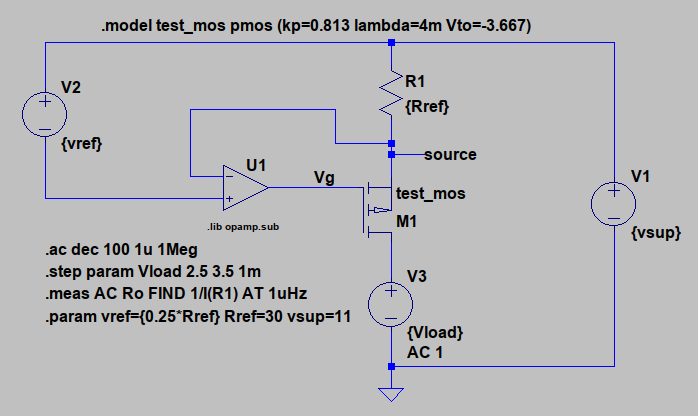
\includegraphics[width=0.8\linewidth]{../images/ltspice_output_impedance.png}
    \caption{LTSpice model.}
    \label{fig:ltspice_output_impedance_example}
\end{figure}

The simulation uses the same MOSFET model as above and adds an ideal op-amp to control the loop. The op-amp model has a open-loop gain of \num{2e6} and a gain-bandwidth product of \qty{10}{\MHz} as can be approximated from the the datasheet of the \device{AD797} \cite{datasheet_AD797} and is also given in table \ref{tab:current_source_parameters}. This leads to a \qty{3}{\dB} corner frequency of \qty{5}{\Hz}, which will be interesting later.

To access the small-signal model the \textbf{.ac} command is used, because LTSpice uses the small-signal model to calculate the ac response of a circuit at a given working point. The command
\begin{lstlisting}[frame=single, xleftmargin=5mm, xrightmargin=5mm, columns=fullflexible, morekeywords={model, ac, dc, options}, keywordstyle=\bfseries, basicstyle=\rmfamily]]
 .ac dec 100 1u 1Meg
\end{lstlisting}
calculates the ac response from \qty{1}{\micro\hertz} to \qty{1}{\MHz} with \qty{100}{points \per decade}.
Additionally, as discussed, the load will be stepped, by stepping voltage source in the source leg of the MOSFET. We use a voltage source in this case instead of a resistor, because the AC impedance of a laser diode is typically very small. For the working point, it does not matter whether $V_{load}$ is resistive or not. To step the voltage source, the command
\begin{lstlisting}[frame=single, xleftmargin=5mm, xrightmargin=5mm, columns=fullflexible, morekeywords={model, ac, dc, options, step}, keywordstyle=\bfseries, basicstyle=\rmfamily]]
.step param Vload 2.5 3.5 1m
\end{lstlisting}
is used to change $V_{load}$ from \qtyrange{2.5}{3.5}{\V} in steps of \qty{1}{\mV}, which is exactly the maximum $V_{DS}$, which is $V_{sup} - V_{ref} = \qty{3.5}{\V}$. This is done to show the effect of the complete loss of regulation. The last thing to do, is to extract the desired output impedance from the many stepped small-signal simulations. This can be done using the \textbf{.meas} command telling LTSpice to save a single value at certain frequency from each step.
\begin{lstlisting}[frame=single, xleftmargin=5mm, xrightmargin=5mm, columns=fullflexible, morekeywords={model, ac, dc, options, step, meas}, keywordstyle=\bfseries, basicstyle=\rmfamily]]
.meas AC Ro FIND 1/I(R1) AT 1uHz
\end{lstlisting}
The \textbf{.meas} command shown will save the value of $\frac{1}{i_{D}} = \frac{1}{I(R1)}$ at \qty{1}{\micro\hertz} to the (error) log file whenever the \textbf{.ac} command is run. The value of $v_{DS}$ was already set to \qty{1}{\V_{rms}} in the LTSpice simulation as shown in figure \ref{fig:ltspice_output_impedance_example}, thus $\frac{\qty{1}{\V}}{I(R1)} = R_{out}$. The current through sense resistor instead of $i_D$ was chosen because it is numerically more stable and since there is no gate current it is the same as $i_D$. The frequency were the $R_{out}$ is measured was chosen to be well below the corner frequency of the op-gain, which was calculated above to be \qty{5}{\Hz}. This gives the near DC output impedance of the current source.

To plot the values stored in the log file, click on \textit{View} in top menu, then \textit{SPICE Error Log}. Now right-click on the error log and select \textit{Plot stepp'ed .meas data}. This will open a new plot window showing the output impedance curve.

Those results are discussed in more detail in section \ref{sec:compliance_voltage}.



\end{document}

